\documentclass{beamer}\usepackage[]{graphicx}\usepackage[]{color}
%% maxwidth is the original width if it is less than linewidth
%% otherwise use linewidth (to make sure the graphics do not exceed the margin)
\makeatletter
\def\maxwidth{ %
  \ifdim\Gin@nat@width>\linewidth
    \linewidth
  \else
    \Gin@nat@width
  \fi
}
\makeatother

\definecolor{fgcolor}{rgb}{0.345, 0.345, 0.345}
\newcommand{\hlnum}[1]{\textcolor[rgb]{0.686,0.059,0.569}{#1}}%
\newcommand{\hlstr}[1]{\textcolor[rgb]{0.192,0.494,0.8}{#1}}%
\newcommand{\hlcom}[1]{\textcolor[rgb]{0.678,0.584,0.686}{\textit{#1}}}%
\newcommand{\hlopt}[1]{\textcolor[rgb]{0,0,0}{#1}}%
\newcommand{\hlstd}[1]{\textcolor[rgb]{0.345,0.345,0.345}{#1}}%
\newcommand{\hlkwa}[1]{\textcolor[rgb]{0.161,0.373,0.58}{\textbf{#1}}}%
\newcommand{\hlkwb}[1]{\textcolor[rgb]{0.69,0.353,0.396}{#1}}%
\newcommand{\hlkwc}[1]{\textcolor[rgb]{0.333,0.667,0.333}{#1}}%
\newcommand{\hlkwd}[1]{\textcolor[rgb]{0.737,0.353,0.396}{\textbf{#1}}}%

\usepackage{framed}
\makeatletter
\newenvironment{kframe}{%
 \def\at@end@of@kframe{}%
 \ifinner\ifhmode%
  \def\at@end@of@kframe{\end{minipage}}%
  \begin{minipage}{\columnwidth}%
 \fi\fi%
 \def\FrameCommand##1{\hskip\@totalleftmargin \hskip-\fboxsep
 \colorbox{shadecolor}{##1}\hskip-\fboxsep
     % There is no \\@totalrightmargin, so:
     \hskip-\linewidth \hskip-\@totalleftmargin \hskip\columnwidth}%
 \MakeFramed {\advance\hsize-\width
   \@totalleftmargin\z@ \linewidth\hsize
   \@setminipage}}%
 {\par\unskip\endMakeFramed%
 \at@end@of@kframe}
\makeatother

\definecolor{shadecolor}{rgb}{.97, .97, .97}
\definecolor{messagecolor}{rgb}{0, 0, 0}
\definecolor{warningcolor}{rgb}{1, 0, 1}
\definecolor{errorcolor}{rgb}{1, 0, 0}
\newenvironment{knitrout}{}{} % an empty environment to be redefined in TeX

\usepackage{alltt}
\usefonttheme[onlymath]{serif}

\usepackage[portuguese]{babel}
\usepackage{graphicx}
\usepackage{ulem} % Para texto em strikeout
\usepackage{amsmath}
\usepackage{amssymb}

\usetheme{m}

\ifdefined\knitrout 
\renewenvironment{knitrout}{\setlength{\topsep}{0mm}}{}
\else
\fi

\title{Aula 6: Regressão Múltipla, ANOVA e ANCOVA}
\subtitle{Análise Estatística e Modelagem de Dados Ecológicos}
\author{\textbf{Thiago S. F. Silva} - tsfsilva@rc.unesp.br}
\institute{Programa de Pós Graduação em Ecologia e Biodiversidade - UNESP}
\date{\today}

\graphicspath{{C:/Users/thiago/OneDrive/UNESP/Pos_graduacao/Eco/2015/Estatistica_2015/Aulas/Aula_7_Anova/figuras/}}
\IfFileExists{upquote.sty}{\usepackage{upquote}}{}
\begin{document}



%===============================================================================%
\begin{frame}[plain] % plain avoids a badbox error from page number in title page
  \titlepage
\end{frame}

\begin{frame}{Outline}
  \tableofcontents
\end{frame}
%===============================================================================%

\section{Regressão Múltipla}


%===============================================================================%
\begin{frame}{Um é pouco, dois é bom, três é melhor ainda}

O modelo de regressão múltipla é uma extensão do modelo simples 

\vfill

Para duas variáveis explicativas, temos: \pause

\begin{equation*}
Y_i = \beta _0 + \beta _1 X_1 + \beta _2 X_2 + \ldots + \beta _k X_k + \varepsilon _i \pause
\end{equation*}

Os termos fixos nos dão $E(Y)$, e o termo aleatório nos dá $Var(Y)$. \pause

\vfill

Se $E(Y)$ depende de uma combinação de duas variáveis preditoras ($X_1$ e $X_2$), a reta se torna um plano 

\vfill

% Designamos as diferentes variáveis explicativas por $X_1$, $X_2$, \ldots, $X_{(p-1)}$, onde $p$ é o número de parametros (coeficientes) do modelo.

\end{frame}
%===============================================================================%


%===============================================================================%
\begin{frame}{Um é pouco, dois é bom, três é melhor ainda}

\begin{knitrout}
\definecolor{shadecolor}{rgb}{0.969, 0.969, 0.969}\color{fgcolor}
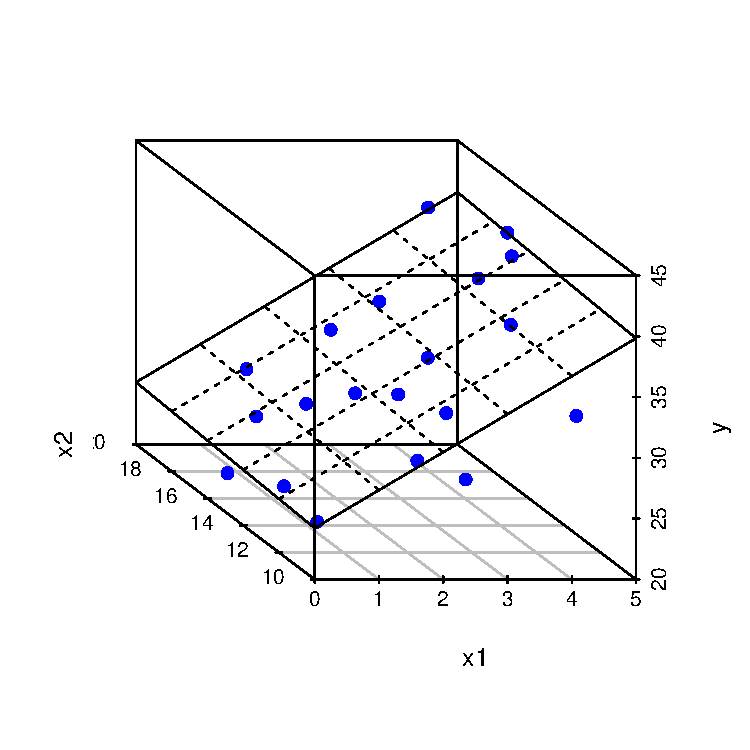
\includegraphics[width=0.8\linewidth]{figure/c1-1} 

\end{knitrout}

\end{frame}
%===============================================================================%


%===============================================================================%
\begin{frame}{Interpretação dos termos do modelo}

\begin{itemize}

\item $\beta _0$: intercepto da superfície de resposta. Valor de $Y$ quando  $X_{1} = X_2 = \dots X_{k=(p-1)} = 0$. Geralmente não tem um significado explícito. \pause
\vfill
\item $\beta _1$, $\beta _2$, \ldots, $\beta _k$: determinam o aumento em $E(Y)$ quando $X_{k}$ $(k=\{0,p-1\})$ aumenta em 1, e os demais $X_k$ permanecem constantes.\pause
\vfill
\item Cada coeficiente representa a contribuição absoluta de  $X_{k}$ para a estimativa de $E(Y)$ (ou $\beta _k = \frac{\delta E(Y)}{\delta X_{(k)}}$) \pause
\vfill
\item $\varepsilon _i$ continua sendo a diferença entre $Y_i$ e $E(Y_i)$

\end{itemize}

\end{frame}
%===============================================================================%

%===============================================================================%
\begin{frame}{Partição da variância}

A partição geral da variância segue o mesmo padrão do modelo simples, mas com diferentes graus de liberdade
\vfill
\resizebox{\textwidth}{!}{%
\begin{tabular}{lcllccc}
Fonte & GL & Soma Quadrados & Média Quadrados \\
\hline
& & & & & &\\
Regressão & $p-1$ & $SQ_{Reg} = \mathbf{b'X'Y-\dfrac{1}{n} Y'JY}$ & $MR_{Reg} = \dfrac{SQ_{Reg}}{p-1}$ \\[5ex]
Resíduos & $n-p$ & $SQ_{Res} = \mathbf{Y'Y - b'X'Y}$ & $MQ_{Res} = \dfrac{SQ_{Res}}{n-p}$ \\[5ex]
Total & $n-1$ & $SQ_{Tot} = \mathbf{Y'Y - \dfrac{1}{n} Y'JY}$ & $MQ_{Tot} = \dfrac{SQ_{Tot}}{n-1}$ \\[5ex]
\hline
\end{tabular}%
}

\end{frame}
%===============================================================================%


%===============================================================================%
\begin{frame}{Coeficiente de determinação múltiplo}

\begin{itemize}

\item O teste geral para a regressão ainda é feito usando $F^* = \frac{MQ_{Reg}}{MQ_{Res}}$, e a quantidade de variância explicada é representada por $R^2 = \frac{SQ_{Reg}}{SQ_{Tot}} = 1 - \frac{SQ_{Res}}{SQ_{Tot}}$ \pause

\vfill

\item Quando novas variáveis são incluídas no modelo, pode-se mostrar matematicamente que $SQ_{Res} nunca aumenta. \pause
\vfill
Por esse motivo, o $R^2$ aumenta mesmo que a quantidade de variância adicional explicada seja mínima. \pause
\vfill
\item Assim, não se pode confiar em $R^2$ como uma medida de qualidade do modelo (a interpretação de quantidade de variância explicada continua correta).


\end{itemize}

\end{frame}
%===============================================================================%


%===============================================================================%
\begin{frame}{Coeficiente de determinação múltiplo}

\begin{itemize}

\item O coeficiente de determinação ajustado ($R^2_a$) penaliza a razão de somas de quadrados pela razão entre os graus de liberdade:

\begin{equation*}
\centering
R ^2 _a = 1 - \left(\frac{n-1}{n-p}\right) \frac{SQ_{Res}}{SQ_{Tot}}

\end{equation*}

\pause
\item Dessa maneira, o ganho em explicação é ponderado pelo aumento de $\frac{(n-1)}{(n-p)}$, e o $R^2_a$ pode até diminuir com a adição de novas variáveis, se a contribuição não for importante.

\vfill

(Mas $R^2_a$ deixa de ter relação com \% de variância explicada)

\end{itemize}

\end{frame}
%===============================================================================%


%===============================================================================%
\begin{frame}{Inferências e Diagnósticos}

As inferências sobre o modelo (intervalos de confiança e testes de hipótese) seguem o mesmo modelo da regressão simples.

\vfill
As equações para estimativas dos erros são mais complexas, mas o princípio não se altera.

\vfill
Os procedimentos diagnósticos também são os mesmos, com a adição de scatterplots dos resíduos verus cada variável $X_k$.

\end{frame}
%===============================================================================%

\section{Diferenças entre Regressão Simples e Múltipla}


%===============================================================================%
\begin{frame}{Complicações adicionais}

Os modelos lineares de regressão múltipla apresentam algumas ``complicações'' extras quando comparados aos modelos simples:
\vfill
\begin{itemize}

\item A existência de correlação entre as variáveis pode atrapalhar a nossa partição de variância (multicolinearidade). \pause
\vfill
\item Os coeficientes $\beta$ normalmente não são diretamente comparáveis. \pause
\vfill
\item Quando o número de variáveis independentes aumenta, a decisão sobre quais são mais ou menos importantes é mais difícil.
\vfill

\end{itemize}

\end{frame}
%===============================================================================%


%===============================================================================%
\begin{frame}{Multicolinearidade}

O modelo de regressão busca explicar parte da variância de $Y$ através da co-variância entre $Y$ e $X$ (partição de variâncias).
\vfill
Se as variáveis $X$ são independentes, cada porção da variância de $Y$ é explicada separadamente por cada $X$.
\vfill
Mas se as variáveis preditoras foem correlacionadas, há redundância de informação, reduzindo a quantidade de informação disponível para estimação dos coeficientes. $\beta$.
\vfill


\end{frame}
%===============================================================================%


%===============================================================================%
\begin{frame}{Multicolinearidade}

Caso 1: $X_k$ perfeitamente independentes
\vfill
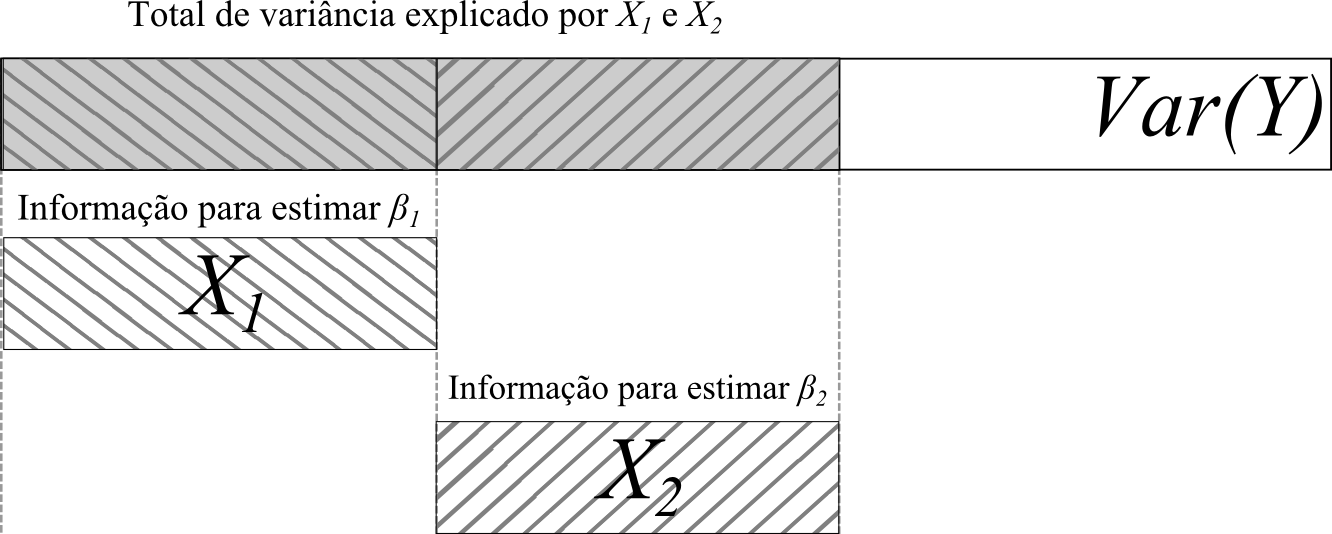
\includegraphics[width=1\textwidth]{multi1.png}


\end{frame}
%===============================================================================%


%===============================================================================%
\begin{frame}[fragile]{Multicolinearidade}

Caso 1: $X_k$ perfeitamente independentes
\vfill
Nesse caso, a contribuição de $X_1$ e $X_2$ são exatamente as mesmas de dois modelos lineares simples:
\vfill
\begin{knitrout}\tiny
\definecolor{shadecolor}{rgb}{0.969, 0.969, 0.969}\color{fgcolor}\begin{kframe}
\begin{alltt}
\hlstd{x1} \hlkwb{<-} \hlkwd{c}\hlstd{(}\hlnum{4}\hlstd{,}\hlnum{4}\hlstd{,}\hlnum{4}\hlstd{,}\hlnum{4}\hlstd{,}\hlnum{6}\hlstd{,}\hlnum{6}\hlstd{,}\hlnum{6}\hlstd{,}\hlnum{6}\hlstd{)}
\hlstd{x2} \hlkwb{<-} \hlkwd{c}\hlstd{(}\hlnum{2}\hlstd{,}\hlnum{2}\hlstd{,}\hlnum{3}\hlstd{,}\hlnum{3}\hlstd{,}\hlnum{2}\hlstd{,}\hlnum{2}\hlstd{,}\hlnum{3}\hlstd{,}\hlnum{3}\hlstd{)}
\hlstd{y} \hlkwb{<-} \hlkwd{c}\hlstd{(}\hlnum{42}\hlstd{,}\hlnum{39}\hlstd{,}\hlnum{48}\hlstd{,}\hlnum{51}\hlstd{,}\hlnum{49}\hlstd{,}\hlnum{53}\hlstd{,}\hlnum{61}\hlstd{,}\hlnum{60}\hlstd{)}

\hlkwd{cor}\hlstd{(x1,x2)}
\end{alltt}
\begin{verbatim}
## [1] 0
\end{verbatim}
\end{kframe}
\end{knitrout}

\end{frame}
%===============================================================================%


%===============================================================================%
\begin{frame}[fragile]{Multicolinearidade}

Caso 1: $X_k$ perfeitamente independentes
\vfill

\begin{knitrout}\tiny
\definecolor{shadecolor}{rgb}{0.969, 0.969, 0.969}\color{fgcolor}\begin{kframe}
\begin{alltt}
\hlstd{m1} \hlkwb{<-} \hlkwd{lm}\hlstd{(y} \hlopt{~} \hlstd{x1)}
\hlstd{m1}
\end{alltt}
\begin{verbatim}
## 
## Call:
## lm(formula = y ~ x1)
## 
## Coefficients:
## (Intercept)           x1  
##      23.500        5.375
\end{verbatim}
\begin{alltt}
\hlkwd{anova}\hlstd{(m1)}
\end{alltt}
\begin{verbatim}
## Analysis of Variance Table
## 
## Response: y
##           Df Sum Sq Mean Sq F value  Pr(>F)  
## x1         1 231.12 231.125   7.347 0.03508 *
## Residuals  6 188.75  31.458                  
## ---
## Signif. codes:  0 '***' 0.001 '**' 0.01 '*' 0.05 '.' 0.1 ' ' 1
\end{verbatim}
\end{kframe}
\end{knitrout}

\end{frame}
%===============================================================================%



%===============================================================================%
\begin{frame}[fragile]{Multicolinearidade}

Caso 1: $X_k$ perfeitamente independentes
\vfill

\begin{knitrout}\tiny
\definecolor{shadecolor}{rgb}{0.969, 0.969, 0.969}\color{fgcolor}\begin{kframe}
\begin{alltt}
\hlstd{m2} \hlkwb{<-} \hlkwd{lm}\hlstd{(y} \hlopt{~} \hlstd{x2)}
\hlstd{m2}
\end{alltt}
\begin{verbatim}
## 
## Call:
## lm(formula = y ~ x2)
## 
## Coefficients:
## (Intercept)           x2  
##       27.25         9.25
\end{verbatim}
\begin{alltt}
\hlkwd{anova}\hlstd{(m2)}
\end{alltt}
\begin{verbatim}
## Analysis of Variance Table
## 
## Response: y
##           Df Sum Sq Mean Sq F value  Pr(>F)  
## x2         1 171.12 171.125  4.1276 0.08846 .
## Residuals  6 248.75  41.458                  
## ---
## Signif. codes:  0 '***' 0.001 '**' 0.01 '*' 0.05 '.' 0.1 ' ' 1
\end{verbatim}
\end{kframe}
\end{knitrout}

\end{frame}
%===============================================================================%


%===============================================================================%
\begin{frame}[fragile]{Multicolinearidade}

Caso 1: $X_k$ perfeitamente independentes
\vfill

\begin{knitrout}\tiny
\definecolor{shadecolor}{rgb}{0.969, 0.969, 0.969}\color{fgcolor}\begin{kframe}
\begin{alltt}
\hlstd{m3} \hlkwb{<-} \hlkwd{lm}\hlstd{(y} \hlopt{~} \hlstd{x1} \hlopt{+} \hlstd{x2)}
\hlstd{m3}
\end{alltt}
\begin{verbatim}
## 
## Call:
## lm(formula = y ~ x1 + x2)
## 
## Coefficients:
## (Intercept)           x1           x2  
##       0.375        5.375        9.250
\end{verbatim}
\begin{alltt}
\hlkwd{anova}\hlstd{(m3)}
\end{alltt}
\begin{verbatim}
## Analysis of Variance Table
## 
## Response: y
##           Df  Sum Sq Mean Sq F value    Pr(>F)    
## x1         1 231.125 231.125  65.567 0.0004657 ***
## x2         1 171.125 171.125  48.546 0.0009366 ***
## Residuals  5  17.625   3.525                      
## ---
## Signif. codes:  0 '***' 0.001 '**' 0.01 '*' 0.05 '.' 0.1 ' ' 1
\end{verbatim}
\end{kframe}
\end{knitrout}

\end{frame}
%===============================================================================%



%===============================================================================%
\begin{frame}{Multicolinearidade}
 
Caso 2: $X_k$ perfeitamente correlacionados
\vfill
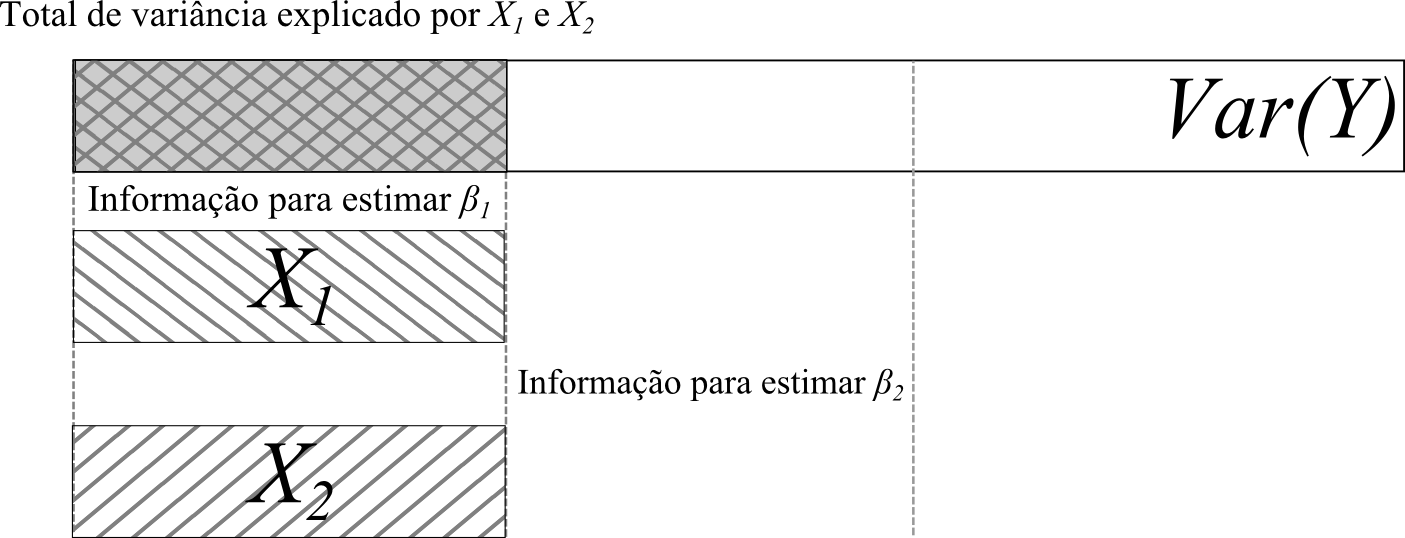
\includegraphics[width=1\textwidth]{multi3v2.png}

\end{frame}
%===============================================================================%

%===============================================================================%
\begin{frame}[fragile]{Multicolinearidade}

Caso 2: $X_k$ perfeitamente correlacionados
\vfill
Nesse caso, não há variância restante para estimar $\beta _2$ após a estimação de $\beta _1$:
\vfill
\begin{knitrout}\tiny
\definecolor{shadecolor}{rgb}{0.969, 0.969, 0.969}\color{fgcolor}\begin{kframe}
\begin{alltt}
\hlstd{x1} \hlkwb{<-} \hlkwd{c}\hlstd{(}\hlnum{4}\hlstd{,}\hlnum{4}\hlstd{,}\hlnum{4}\hlstd{,}\hlnum{4}\hlstd{,}\hlnum{6}\hlstd{,}\hlnum{6}\hlstd{,}\hlnum{6}\hlstd{,}\hlnum{6}\hlstd{)}
\hlstd{x2} \hlkwb{<-} \hlstd{x1}
\hlstd{y} \hlkwb{<-} \hlkwd{c}\hlstd{(}\hlnum{42}\hlstd{,}\hlnum{39}\hlstd{,}\hlnum{48}\hlstd{,}\hlnum{51}\hlstd{,}\hlnum{49}\hlstd{,}\hlnum{53}\hlstd{,}\hlnum{61}\hlstd{,}\hlnum{60}\hlstd{)}

\hlkwd{cor}\hlstd{(x1,x2)}
\end{alltt}
\begin{verbatim}
## [1] 1
\end{verbatim}
\end{kframe}
\end{knitrout}

\end{frame}
%===============================================================================%


%===============================================================================%
\begin{frame}[fragile]{Multicolinearidade}

Caso 2: $X_k$ perfeitamente correlacionados
\vfill

\begin{knitrout}\tiny
\definecolor{shadecolor}{rgb}{0.969, 0.969, 0.969}\color{fgcolor}\begin{kframe}
\begin{alltt}
\hlstd{m1} \hlkwb{<-} \hlkwd{lm}\hlstd{(y} \hlopt{~} \hlstd{x1} \hlopt{+} \hlstd{x2)}
\hlstd{m1}
\end{alltt}
\begin{verbatim}
## 
## Call:
## lm(formula = y ~ x1 + x2)
## 
## Coefficients:
## (Intercept)           x1           x2  
##      23.500        5.375           NA
\end{verbatim}
\begin{alltt}
\hlkwd{anova}\hlstd{(m1)}
\end{alltt}
\begin{verbatim}
## Analysis of Variance Table
## 
## Response: y
##           Df Sum Sq Mean Sq F value  Pr(>F)  
## x1         1 231.12 231.125   7.347 0.03508 *
## Residuals  6 188.75  31.458                  
## ---
## Signif. codes:  0 '***' 0.001 '**' 0.01 '*' 0.05 '.' 0.1 ' ' 1
\end{verbatim}
\end{kframe}
\end{knitrout}

\end{frame}
%===============================================================================%

%===============================================================================%
\begin{frame}[fragile]{Multicolinearidade}

Caso 2: $X_k$ perfeitamente correlacionados
\vfill

\begin{knitrout}\tiny
\definecolor{shadecolor}{rgb}{0.969, 0.969, 0.969}\color{fgcolor}\begin{kframe}
\begin{alltt}
\hlstd{m2} \hlkwb{<-} \hlkwd{lm}\hlstd{(y} \hlopt{~} \hlstd{x2} \hlopt{+} \hlstd{x1)}
\hlstd{m2}
\end{alltt}
\begin{verbatim}
## 
## Call:
## lm(formula = y ~ x2 + x1)
## 
## Coefficients:
## (Intercept)           x2           x1  
##      23.500        5.375           NA
\end{verbatim}
\begin{alltt}
\hlkwd{anova}\hlstd{(m2)}
\end{alltt}
\begin{verbatim}
## Analysis of Variance Table
## 
## Response: y
##           Df Sum Sq Mean Sq F value  Pr(>F)  
## x2         1 231.12 231.125   7.347 0.03508 *
## Residuals  6 188.75  31.458                  
## ---
## Signif. codes:  0 '***' 0.001 '**' 0.01 '*' 0.05 '.' 0.1 ' ' 1
\end{verbatim}
\end{kframe}
\end{knitrout}

\end{frame}
%===============================================================================%


%===============================================================================%
\begin{frame}{Multicolinearidade}

Caso 3: $X_k$ parcialmente correlacionados
\vfill
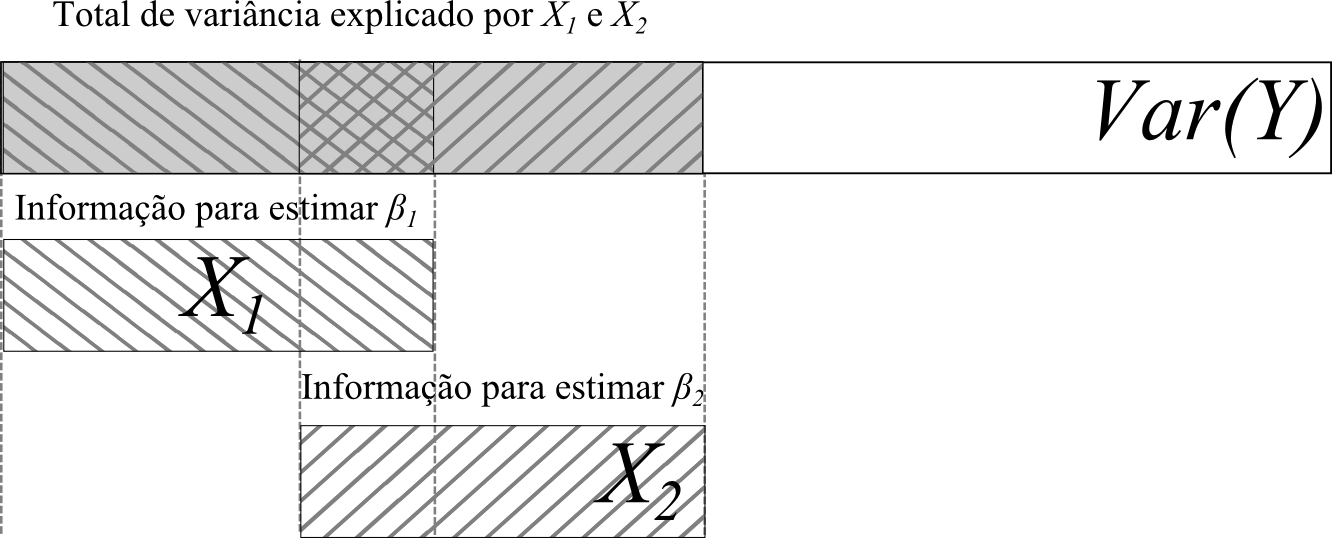
\includegraphics[width=1\textwidth]{multi2.png}
 
\end{frame}
%===============================================================================%


%===============================================================================%
\begin{frame}[fragile]{Multicolinearidade}

Caso 3: $X_k$ parcialmente correlacionados
\vfill
Nesse caso, há "menos" variância restante para estimar $\beta _2$ após a estimação de $\beta _1$:
\vfill
\begin{knitrout}\tiny
\definecolor{shadecolor}{rgb}{0.969, 0.969, 0.969}\color{fgcolor}\begin{kframe}
\begin{alltt}
\hlstd{x1} \hlkwb{<-} \hlkwd{c}\hlstd{(}\hlnum{4}\hlstd{,}\hlnum{4}\hlstd{,}\hlnum{4}\hlstd{,}\hlnum{4}\hlstd{,}\hlnum{6}\hlstd{,}\hlnum{6}\hlstd{,}\hlnum{6}\hlstd{,}\hlnum{6}\hlstd{)}
\hlkwd{set.seed}\hlstd{(}\hlnum{154}\hlstd{)}
\hlstd{x2} \hlkwb{<-} \hlstd{x1} \hlopt{+} \hlkwd{runif}\hlstd{(}\hlnum{8}\hlstd{,}\hlnum{0}\hlstd{,}\hlnum{1}\hlstd{)}
\hlstd{y} \hlkwb{<-} \hlkwd{c}\hlstd{(}\hlnum{42}\hlstd{,}\hlnum{39}\hlstd{,}\hlnum{48}\hlstd{,}\hlnum{51}\hlstd{,}\hlnum{49}\hlstd{,}\hlnum{53}\hlstd{,}\hlnum{61}\hlstd{,}\hlnum{60}\hlstd{)}

\hlkwd{cor}\hlstd{(x1,x2)}
\end{alltt}
\begin{verbatim}
## [1] 0.9592065
\end{verbatim}
\end{kframe}
\end{knitrout}

\end{frame}
%===============================================================================%


%===============================================================================%
\begin{frame}[fragile]{Multicolinearidade}

Caso 3: $X_k$ parcialmente correlacionados
\vfill

\begin{knitrout}\tiny
\definecolor{shadecolor}{rgb}{0.969, 0.969, 0.969}\color{fgcolor}\begin{kframe}
\begin{alltt}
\hlstd{m1} \hlkwb{<-} \hlkwd{lm}\hlstd{(y} \hlopt{~} \hlstd{x1} \hlopt{+} \hlstd{x2)}
\hlstd{m1}
\end{alltt}
\begin{verbatim}
## 
## Call:
## lm(formula = y ~ x1 + x2)
## 
## Coefficients:
## (Intercept)           x1           x2  
##      23.886        6.878       -1.418
\end{verbatim}
\begin{alltt}
\hlkwd{anova}\hlstd{(m1)}
\end{alltt}
\begin{verbatim}
## Analysis of Variance Table
## 
## Response: y
##           Df Sum Sq Mean Sq F value  Pr(>F)  
## x1         1 231.12 231.125  6.1739 0.05552 .
## x2         1   1.57   1.570  0.0419 0.84583  
## Residuals  5 187.18  37.436                  
## ---
## Signif. codes:  0 '***' 0.001 '**' 0.01 '*' 0.05 '.' 0.1 ' ' 1
\end{verbatim}
\end{kframe}
\end{knitrout}

\end{frame}
%===============================================================================%

%===============================================================================%
\begin{frame}[fragile]{Multicolinearidade}

Caso 3: $X_k$ parcialmente correlacionados
\vfill

\begin{knitrout}\tiny
\definecolor{shadecolor}{rgb}{0.969, 0.969, 0.969}\color{fgcolor}\begin{kframe}
\begin{alltt}
\hlstd{m2} \hlkwb{<-} \hlkwd{lm}\hlstd{(y} \hlopt{~} \hlstd{x2} \hlopt{+} \hlstd{x1)}
\hlstd{m2}
\end{alltt}
\begin{verbatim}
## 
## Call:
## lm(formula = y ~ x2 + x1)
## 
## Coefficients:
## (Intercept)           x2           x1  
##      23.886       -1.418        6.878
\end{verbatim}
\begin{alltt}
\hlkwd{anova}\hlstd{(m2)}
\end{alltt}
\begin{verbatim}
## Analysis of Variance Table
## 
## Response: y
##           Df  Sum Sq Mean Sq F value  Pr(>F)  
## x2         1 202.448 202.448  5.4078 0.06759 .
## x1         1  30.246  30.246  0.8080 0.40992  
## Residuals  5 187.180  37.436                  
## ---
## Signif. codes:  0 '***' 0.001 '**' 0.01 '*' 0.05 '.' 0.1 ' ' 1
\end{verbatim}
\end{kframe}
\end{knitrout}

\end{frame}
%===============================================================================%



%===============================================================================%
\begin{frame}{Multicolinearidade}

Que parte do modelo de regressão esperamos que vá ser afetada pela multicolinearidade?  \pause

\begin{itemize}

\item Os coeficientes $\beta _1$, \ldots, $\beta _k$ \pause

\end{itemize}

Qual será o principal efeito da multicolinearidade sobre a especificação do modelo? \pause

\begin{itemize}

\item As propriedades dos estimadores não se alteram (\emph{BLUE}) \pause

\item Devido à redução na quantidade de informação disponível, o erro de cada $b_k$ aumenta \pause

\item Como a informação é redudante, múltiplas combinações de $X_k$ e $b_k$ podem dar o mesmo resultado final 
 
\end{itemize}

\end{frame}
%===============================================================================%


%===============================================================================%
\begin{frame}[fragile]{Exemplo}

\begin{knitrout}\tiny
\definecolor{shadecolor}{rgb}{0.969, 0.969, 0.969}\color{fgcolor}\begin{kframe}
\begin{alltt}
\hlkwd{set.seed}\hlstd{(}\hlnum{1500}\hlstd{)}
\hlstd{x1} \hlkwb{<-} \hlkwd{runif}\hlstd{(}\hlnum{50}\hlstd{,}\hlnum{0}\hlstd{,}\hlnum{20}\hlstd{)}
\hlstd{x2} \hlkwb{<-} \hlstd{x1} \hlopt{+} \hlkwd{runif}\hlstd{(}\hlnum{50}\hlstd{,}\hlnum{0}\hlstd{,}\hlnum{5}\hlstd{)}
\hlstd{y} \hlkwb{<-} \hlnum{24} \hlopt{+} \hlnum{1.2} \hlopt{*}\hlstd{x1} \hlopt{+} \hlnum{2.1}\hlopt{*}\hlstd{x2} \hlopt{+} \hlkwd{rnorm}\hlstd{(}\hlnum{50}\hlstd{,}\hlnum{0}\hlstd{,}\hlnum{20}\hlstd{)}
\hlstd{m1} \hlkwb{<-} \hlkwd{lm}\hlstd{(y} \hlopt{~} \hlstd{x1)}
\hlkwd{summary}\hlstd{(m1)}
\end{alltt}
\begin{verbatim}
## 
## Call:
## lm(formula = y ~ x1)
## 
## Residuals:
##     Min      1Q  Median      3Q     Max 
## -49.567 -12.840   1.822  12.161  46.037 
## 
## Coefficients:
##             Estimate Std. Error t value Pr(>|t|)    
## (Intercept)  33.7099     5.6739   5.941 3.08e-07 ***
## x1            3.0194     0.4763   6.339 7.61e-08 ***
## ---
## Signif. codes:  0 '***' 0.001 '**' 0.01 '*' 0.05 '.' 0.1 ' ' 1
## 
## Residual standard error: 19.93 on 48 degrees of freedom
## Multiple R-squared:  0.4556,	Adjusted R-squared:  0.4443 
## F-statistic: 40.18 on 1 and 48 DF,  p-value: 7.607e-08
\end{verbatim}
\end{kframe}
\end{knitrout}


\end{frame}
%===============================================================================%

%===============================================================================%
\begin{frame}[fragile]{Exemplo}

\begin{knitrout}\tiny
\definecolor{shadecolor}{rgb}{0.969, 0.969, 0.969}\color{fgcolor}\begin{kframe}
\begin{alltt}
\hlstd{m2} \hlkwb{<-} \hlkwd{lm}\hlstd{(y} \hlopt{~} \hlstd{x2)}
\hlkwd{summary}\hlstd{(m2)}
\end{alltt}
\begin{verbatim}
## 
## Call:
## lm(formula = y ~ x2)
## 
## Residuals:
##     Min      1Q  Median      3Q     Max 
## -46.280 -11.190  -3.074  10.861  42.214 
## 
## Coefficients:
##             Estimate Std. Error t value Pr(>|t|)    
## (Intercept)  26.9196     6.3456   4.242    1e-04 ***
## x2            2.9624     0.4456   6.649 2.54e-08 ***
## ---
## Signif. codes:  0 '***' 0.001 '**' 0.01 '*' 0.05 '.' 0.1 ' ' 1
## 
## Residual standard error: 19.49 on 48 degrees of freedom
## Multiple R-squared:  0.4794,	Adjusted R-squared:  0.4686 
## F-statistic: 44.21 on 1 and 48 DF,  p-value: 2.541e-08
\end{verbatim}
\end{kframe}
\end{knitrout}


\end{frame}
%===============================================================================%

%===============================================================================%
\begin{frame}[fragile]{Exemplo}

\begin{knitrout}\tiny
\definecolor{shadecolor}{rgb}{0.969, 0.969, 0.969}\color{fgcolor}\begin{kframe}
\begin{alltt}
\hlstd{m3} \hlkwb{<-} \hlkwd{lm}\hlstd{(y} \hlopt{~} \hlstd{x1} \hlopt{+} \hlstd{x2)}
\hlkwd{summary}\hlstd{(m3)}
\end{alltt}
\begin{verbatim}
## 
## Call:
## lm(formula = y ~ x1 + x2)
## 
## Residuals:
##     Min      1Q  Median      3Q     Max 
## -46.823 -11.745  -3.351  10.786  41.832 
## 
## Coefficients:
##             Estimate Std. Error t value Pr(>|t|)    
## (Intercept)  27.4629     7.0189   3.913 0.000293 ***
## x1            0.3541     1.8629   0.190 0.850079    
## x2            2.6348     1.7818   1.479 0.145895    
## ---
## Signif. codes:  0 '***' 0.001 '**' 0.01 '*' 0.05 '.' 0.1 ' ' 1
## 
## Residual standard error: 19.69 on 47 degrees of freedom
## Multiple R-squared:  0.4798,	Adjusted R-squared:  0.4577 
## F-statistic: 21.68 on 2 and 47 DF,  p-value: 2.134e-07
\end{verbatim}
\end{kframe}
\end{knitrout}


\end{frame}
%===============================================================================%



%===============================================================================%
\begin{frame}{Multicolinearidade: diagnóstico}

\begin{small}

Podemos quantificar a existência de multicolinearidade através da medida de \textbf{tolerância}:

\vfill

$T = 1 - R^2_k$ \pause

\vfill

$R^2_k$ vem da regressão $\mathbf{X_k} = \beta _0 + \beta _1 X_1 + \ldots + \beta _{k-1} X_{k-1} + \varepsilon$ \pause

\vfill
Normalmente, expressamos a tolerância na forma inversa, o que denominamos \textbf{Fator de Inflação da Variância} (\emph{Variance Inflation Factor, VIF})

\vfill

$VIF = \dfrac{1}{T} = \dfrac{1}{1-R^2 _k}$ \pause
\vfill

O $VIF$ nos dá a proporção do quanto o erro é "inflado" pela variável. Se $X_k$ tem um $VIF$ de 1.8, isso significa que o erro do coeficiente $b _k$ é 80\% maior do que o esperado se não houvesse colinearidade.

\end{small}

\end{frame}
%===============================================================================%


%===============================================================================%
\begin{frame}[fragile]{Multicolinearidade: diagnóstico}

\begin{knitrout}\tiny
\definecolor{shadecolor}{rgb}{0.969, 0.969, 0.969}\color{fgcolor}\begin{kframe}
\begin{alltt}
\hlkwd{library}\hlstd{(car)}
\hlkwd{vif}\hlstd{(m3)}
\end{alltt}
\begin{verbatim}
##       x1       x2 
## 15.67194 15.67194
\end{verbatim}
\end{kframe}
\end{knitrout}


\end{frame}
%===============================================================================%


%===============================================================================%
\begin{frame}{Multicolinearidade: diagnóstico}

A partir de que valor devemos nos preocupar com o VIF? \pause
\vfill
Não existe uma regra fixa, mas em geral: \pause
\vfill
VIF > 4 pede que a correlação entre os preditores seja melhor investigada \pause
\vfill
VIF > 10 representa multicolinearidade severa, precisa ser corrigida de qualquer maneira 

\end{frame}
%===============================================================================%


%===============================================================================%
\begin{frame}[fragile]{Multicolinearidade: remediação}

 Podemos resolver o problema da multicolinearidade de diversas maneiras: \pause

\vfill

1) Através de uma combinação entre as variáveis (ex.: $X_1 + X_2$) \pause
\vfill
2) Usando os resíduos da regressão entre $X_1$ e $X_2$ \pause
\vfill
3) Ortogonalização (ex.: análise de componentes principais)
 

\end{frame}
%===============================================================================%


%===============================================================================%
\begin{frame}[fragile]{Multicolinearidade: remediação}

1) Através de uma combinação entre as variáveis (ex.: $X_1 + X_2$)
 
\begin{knitrout}\tiny
\definecolor{shadecolor}{rgb}{0.969, 0.969, 0.969}\color{fgcolor}\begin{kframe}
\begin{alltt}
\hlstd{x.novo} \hlkwb{<-} \hlstd{x1} \hlopt{+} \hlstd{x2}
\hlstd{m4} \hlkwb{<-} \hlkwd{lm}\hlstd{(y} \hlopt{~} \hlstd{x.novo)}
\hlkwd{summary}\hlstd{(m4)}
\end{alltt}
\begin{verbatim}
## 
## Call:
## lm(formula = y ~ x.novo)
## 
## Residuals:
##     Min      1Q  Median      3Q     Max 
## -48.328 -13.047  -1.519  11.687  43.449 
## 
## Coefficients:
##             Estimate Std. Error t value Pr(>|t|)    
## (Intercept)  29.7061     6.0136   4.940 9.89e-06 ***
## x.novo        1.5202     0.2305   6.596 3.07e-08 ***
## ---
## Signif. codes:  0 '***' 0.001 '**' 0.01 '*' 0.05 '.' 0.1 ' ' 1
## 
## Residual standard error: 19.56 on 48 degrees of freedom
## Multiple R-squared:  0.4754,	Adjusted R-squared:  0.4645 
## F-statistic:  43.5 on 1 and 48 DF,  p-value: 3.066e-08
\end{verbatim}
\end{kframe}
\end{knitrout}
 

\end{frame}
%===============================================================================%



%===============================================================================%
\begin{frame}[fragile]{Multicolinearidade: remediação}

2) Usando os resíduos da regressão entre $X_1$ e $X_2$

 
\begin{knitrout}\tiny
\definecolor{shadecolor}{rgb}{0.969, 0.969, 0.969}\color{fgcolor}\begin{kframe}
\begin{alltt}
\hlstd{mx} \hlkwb{<-} \hlkwd{lm}\hlstd{(x2} \hlopt{~} \hlstd{x1)}
\hlstd{rx} \hlkwb{<-} \hlkwd{residuals}\hlstd{(mx)}
\hlstd{m5} \hlkwb{<-} \hlkwd{lm}\hlstd{(y} \hlopt{~} \hlstd{x1} \hlopt{+} \hlstd{rx)}
\hlkwd{summary}\hlstd{(m5)}
\end{alltt}
\begin{verbatim}
## 
## Call:
## lm(formula = y ~ x1 + rx)
## 
## Residuals:
##     Min      1Q  Median      3Q     Max 
## -46.823 -11.745  -3.351  10.786  41.832 
## 
## Coefficients:
##             Estimate Std. Error t value Pr(>|t|)    
## (Intercept)  33.7099     5.6050   6.014 2.56e-07 ***
## x1            3.0194     0.4706   6.416 6.29e-08 ***
## rx            2.6348     1.7818   1.479    0.146    
## ---
## Signif. codes:  0 '***' 0.001 '**' 0.01 '*' 0.05 '.' 0.1 ' ' 1
## 
## Residual standard error: 19.69 on 47 degrees of freedom
## Multiple R-squared:  0.4798,	Adjusted R-squared:  0.4577 
## F-statistic: 21.68 on 2 and 47 DF,  p-value: 2.134e-07
\end{verbatim}
\end{kframe}
\end{knitrout}
 

\end{frame}
%===============================================================================%



%===============================================================================%
\begin{frame}[fragile]{Multicolinearidade: remediação}

3) Ortogonalização (ex.: análise de componentes principais)

 
\begin{knitrout}\tiny
\definecolor{shadecolor}{rgb}{0.969, 0.969, 0.969}\color{fgcolor}\begin{kframe}
\begin{alltt}
\hlstd{pca} \hlkwb{<-} \hlkwd{princomp}\hlstd{(}\hlopt{~} \hlstd{x2} \hlopt{+} \hlstd{x1)}
\hlstd{m6} \hlkwb{<-} \hlkwd{lm}\hlstd{(y} \hlopt{~} \hlstd{pca}\hlopt{$}\hlstd{scores[,}\hlnum{1}\hlstd{]} \hlopt{+} \hlstd{pca}\hlopt{$}\hlstd{scores[,}\hlnum{2}\hlstd{])}
\hlkwd{summary}\hlstd{(m6)}
\end{alltt}
\begin{verbatim}
## 
## Call:
## lm(formula = y ~ pca$scores[, 1] + pca$scores[, 2])
## 
## Residuals:
##     Min      1Q  Median      3Q     Max 
## -46.823 -11.745  -3.351  10.786  41.832 
## 
## Coefficients:
##                 Estimate Std. Error t value Pr(>|t|)    
## (Intercept)      64.9237     2.7841  23.319  < 2e-16 ***
## pca$scores[, 1]  -2.1499     0.3279  -6.556 3.86e-08 ***
## pca$scores[, 2]   1.5637     2.5569   0.612    0.544    
## ---
## Signif. codes:  0 '***' 0.001 '**' 0.01 '*' 0.05 '.' 0.1 ' ' 1
## 
## Residual standard error: 19.69 on 47 degrees of freedom
## Multiple R-squared:  0.4798,	Adjusted R-squared:  0.4577 
## F-statistic: 21.68 on 2 and 47 DF,  p-value: 2.134e-07
\end{verbatim}
\end{kframe}
\end{knitrout}
 

\end{frame}
%===============================================================================%


\section{ANOVA: Análise de Variância}



%===============================================================================%
\begin{frame}{ANOVA: Análise de Variância}

A ANOVA pode ser vista como uma regressão usando uma variável $X$ categórica \pause
\vfill
Como $X$ não é contínua, o foco é determinar se existem diferenças em $E(Y)$ para cada nível de $X$, sem a pressuposição de relação linear entre $X$ e$Y$\pause
\vfill
ANOVA e Regressão Linear são casos específicos dos chamados Modelos Lineares Gerais 

\end{frame}
%===============================================================================%



%===============================================================================%
\begin{frame}{ANOVA: Análise de Variância}

\begin{columns}[c]

\column{0.5\linewidth}


\begin{knitrout}
\definecolor{shadecolor}{rgb}{0.969, 0.969, 0.969}\color{fgcolor}
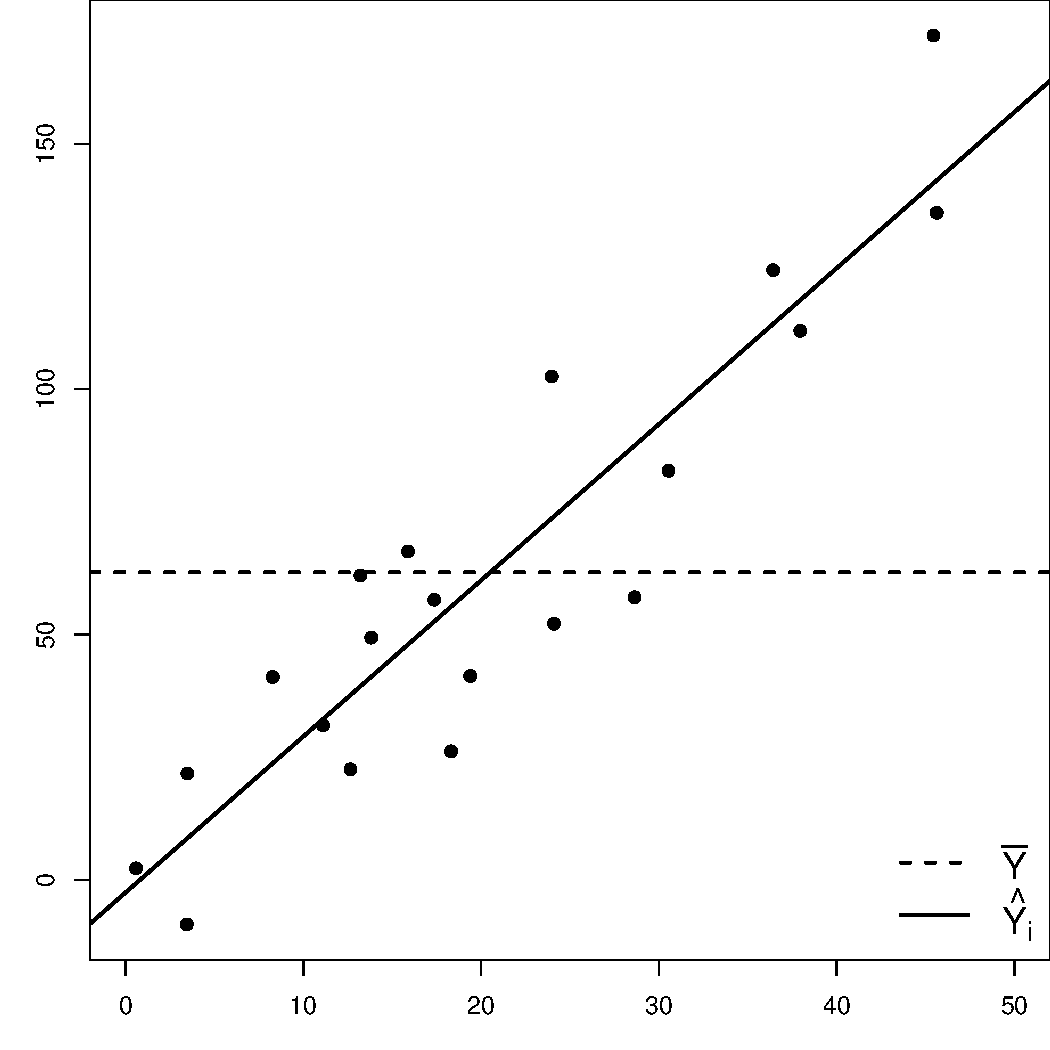
\includegraphics[width=\maxwidth]{figure/unnamed-chunk-1-1} 

\end{knitrout}

\pause

\column{0.5\linewidth}

\begin{knitrout}
\definecolor{shadecolor}{rgb}{0.969, 0.969, 0.969}\color{fgcolor}
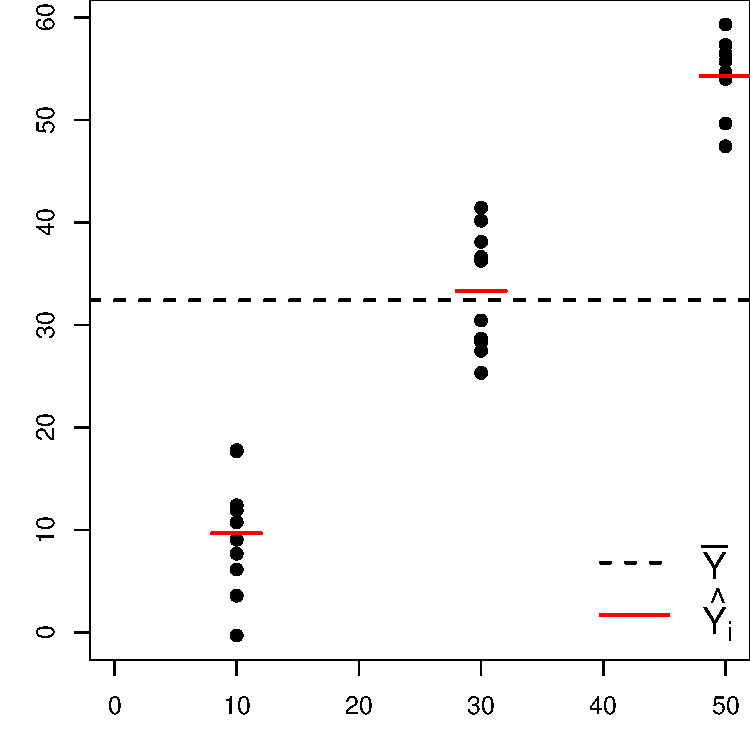
\includegraphics[width=1\linewidth]{figure/plotanova-1} 

\end{knitrout}

\end{columns}

\end{frame}
%===============================================================================%

%===============================================================================%
\begin{frame}{ANOVA: Análise de Variância}

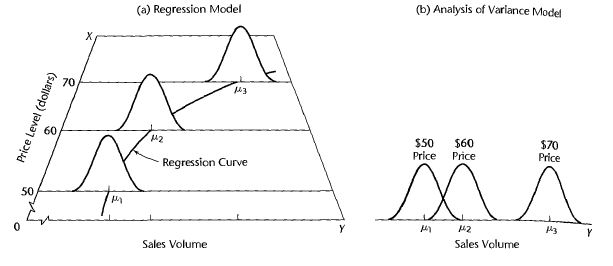
\includegraphics[width = 1\linewidth]{Fig_1.jpg}

\end{frame}
%===============================================================================%


%===============================================================================%
\begin{frame}{ANOVA: Terminologia}

A notação matemática utilizada para a ANOVA é um pouco diferente da regressão: \pause
\vfill
\begin{itemize}
  \item $Y$ ainda é a variável resposta  \pause
  \vfill
  \item Em vez de ter um $X$ contínuo, temos um $X$ categórico (fator), com diferentes níveis ou \emph{tratamentos} que são identificados por $i = (1,2,\ldots,r)$ \pause
  \vfill
  \item Cada $X_i$ tem um certo número de observações, $n_i$, e o número total de obseravções é $n$
    \vfill
  \item Como agora usamos $i$ para identificar os níveis de $X$, usamos $j$ para descrever uma observação específica em cada nível: $j = (1,2,\dots,n_i)$
\end{itemize}

\end{frame}
%===============================================================================%


%===============================================================================%
\begin{frame}{O modelo ANOVA}

O nosso modelo de regressão era:
\vfill

$Y_i = \beta _0 + \beta _1 X_i + \varepsilon_i$ \pause
\vfill

O modelo ANOVA é parecido, mas tem menos parâmetros:
\vfill

$Y_{ij} = \mu_i + \varepsilon _{ij}$ \pause
\vfill
Ou seja, cada valor de $Y$ ($Y_{ij}$) é determinado pela média do grupo $i$, mais um erro aleatório (distância entre $Y_{ij}$ e $\mu _i$). Este é o chamado ``modelo celular'', ou modelo de médias celulares.

\end{frame}
%===============================================================================%

%===============================================================================%
\begin{frame}{O modelo ANOVA}

Também podemos especificar o modelo da seguinte maneira:
\vfill
$Y_{ij} = \mu + \alpha _i + \varepsilon _{ij}$ \pause
\vfill
Aqui, cada valor de $Y$ ($Y_{ij}$) é determinado pela média global de $Y$ ($\mu$), somada ou subtraída de um coeficiente $\alpha$ que varia de acordo com o nível $i$, mais um erro aleatório. ($\mu + \alpha _i = \mu _i$). \pause
\vfill
Este modelo é chamado de ``modelo de efeitos'', já que individualiza os efeitos de cada tratamento.

\end{frame}
%===============================================================================%

%===============================================================================%
\begin{frame}{ANOVA: Análise de Variância}

\begin{columns}[c]

\column{0.5\linewidth}

\begin{knitrout}
\definecolor{shadecolor}{rgb}{0.969, 0.969, 0.969}\color{fgcolor}
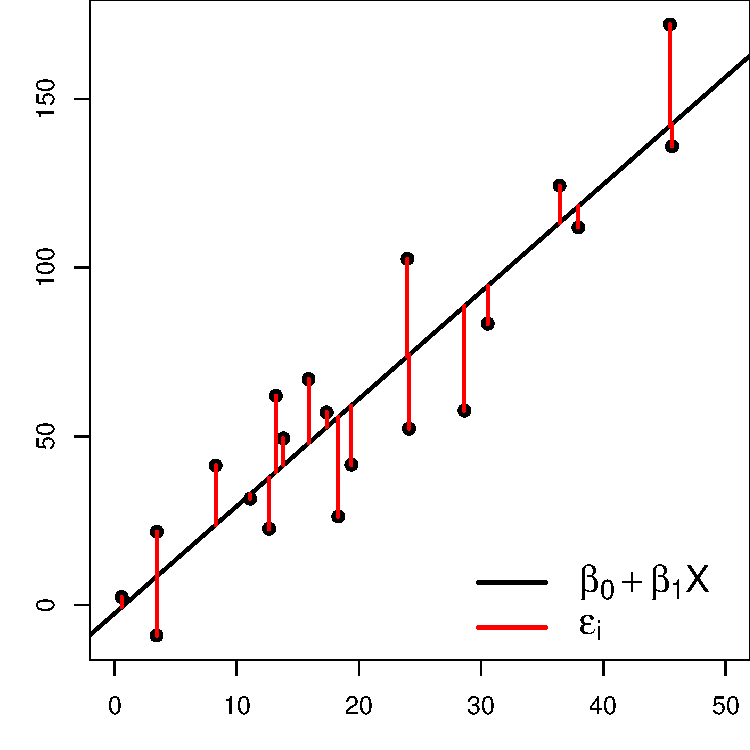
\includegraphics[width=1\linewidth]{figure/plotreg2-1} 

\end{knitrout}

\pause

\column{0.5\linewidth}

\begin{knitrout}
\definecolor{shadecolor}{rgb}{0.969, 0.969, 0.969}\color{fgcolor}
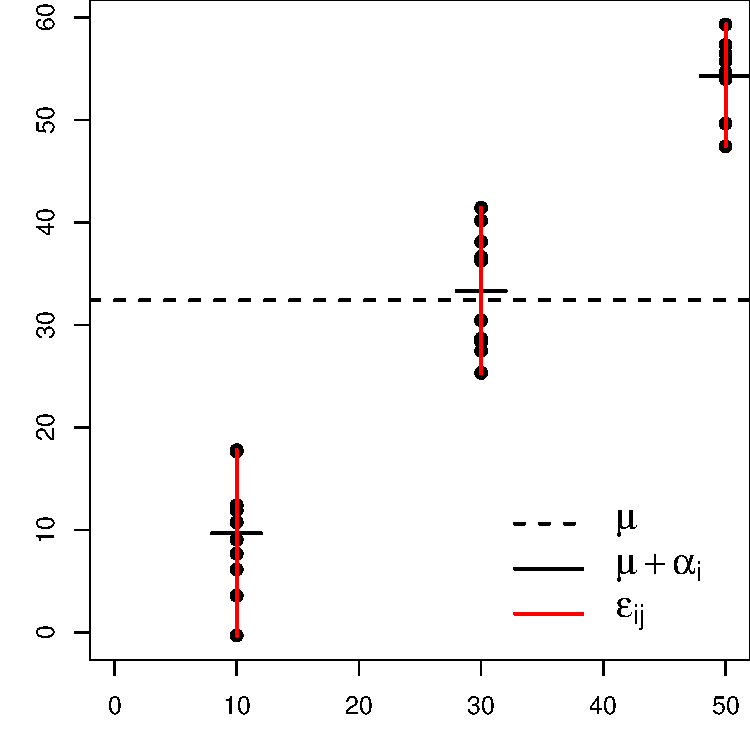
\includegraphics[width=1\linewidth]{figure/plotanova2-1} 

\end{knitrout}

\end{columns}

\end{frame}
%===============================================================================%

%===============================================================================%
\begin{frame}{Pressuposições do modelo ANOVA}

O modelo ANOVA segue pressuposições similares ao modelo de regressão: \pause
\vfill
\begin{itemize}
  \item A distribuição dos erros segue $\varepsilon \sim N(0,\sigma ^2) \pause
  \vfill
  \item $\sigma ^2$ é constante para todos os $i$ níveis de $X$ ($\sigma ^2 _1 = \sigma ^2 _2 \ldots = \sigma ^2 _i = \sigma ^2$) \pause
  \vfill
  \item Os erros $\varepsilon _i$ são independentes entre si \pause
\end{itemize}
\vfill
Se essas pressuposições são verdadeiras, então:
\vfill
$E(Y_{ij}) = \mu + \alpha _i$, $Var(Y_{ij}) = \sigma ^2$
\end{frame}
%===============================================================================%




%===============================================================================%
\begin{frame}{ANOVA: estimando o modelo}

Podemos desdobrar nosso modelo ANOVA para que se assemelhe a uma regressão. No caso de uma ANOVA com três níveis de $X$:
\vfill
$Y_{ij} = \mu + \alpha _i + \varepsilon _{ij}$ \pause
\vfill
$Y_{ij} = \mu + \alpha _1 X_{i=1} + \alpha _2 X_{i=2} + \alpha _3 X_{i=3} + \varepsilon _{ij}$  ou \pause
\vfill
$Y_{ij} = \mu_1 + \alpha _2 X_{i=2} + \alpha _3 X_{i=3} + \varepsilon _{ij}$ \pause
\vfill
Nesse caso, $X_i$ é chamado de variável \textbf{indicadora} (ou \emph{dummy}) com valor $X_i = 1$ para $Y = Y_{ij}$, e $X_i = 0$ quando $Y \neq Y_{ij}$


\end{frame}
%===============================================================================%


%===============================================================================%
\begin{frame}{Exemplo: variável indicadora}

\begin{columns}[c]

\column{0.5\linewidth}

\begin{tabular}{rrl}
  \hline
  $Y$ & $X$ \\ 
  \hline
  62.00 & $A$ \\ 
  60.00 & $A$ \\ 
  63.00 & $A$ \\ 
  63.00 & $B$ \\ 
  67.00 & $B$ \\ 
  71.00 & $B$ \\ 
  72.00 & $C$ \\ 
  70.00 & $C$ \\ 
  75.00 & $C$ \\ 
  \hline
\end{tabular}

\column{0.5\linewidth}

$A = X_{i=1}$
\vfill
$B = X_{i=2}$
\vfill
$C = X_{i=3}$

\end{columns}

\end{frame}
%===============================================================================%


%===============================================================================%
\begin{frame}{Exemplo: variável indicadora}

\begin{columns}[c]

\column{0.4\linewidth}

\begin{tabular}{cc|ccc}
  \hline
  $Y$ & $X$ & $X_1$ & $X_2$ & $X_3$\\ 
  \hline
  62.00 & $A$ & 1 & 0 & 0\\ 
  60.00 & $A$ & 1 & 0 & 0\\ 
  63.00 & $A$ & 1 & 0 & 0\\ 
  63.00 & $B$ & 0 & 1 & 0\\ 
  67.00 & $B$ & 0 & 1 & 0\\ 
  71.00 & $B$ & 0 & 1 & 0\\ 
  72.00 & $C$ & 0 & 0 & 1\\ 
  70.00 & $C$ & 0 & 0 & 1\\ 
  75.00 & $C$ & 0 & 0 & 1\\ 
  \hline
\end{tabular}
\pause
\column{0.6\linewidth}
\vbox to .7\textheight{%

$Y_{ij} = \mu + \alpha _1 X_1 + \alpha _2 X_2 + \alpha _3X_3 + \varepsilon _{ij}$ \pause
\vfill
Para $Y = Y_{Aj}:
\vfill
$Y_{Aj} = \mu + \alpha _1 \times 1 + \alert{\alpha _2 \times 0} + \alert{\alpha _3 \times 0} + \varepsilon _{Aj}$ 
$Y_{Aj} = \mu + \alpha _1 + \varepsilon _{Aj}$ \pause
\vfill
Para $Y = Y_{Bj}:
\vfill
$Y_{Bj} = \mu + \alert{\alpha _1 \times 0} + \alpha _2 \times 1 + \alert{\alpha _3 \times 0} + \varepsilon _{Bj}$ 
$Y_{Bj} = \mu + \alpha _2 + \varepsilon _{Bj}$ \pause
\vfill
Para $Y = Y_{Cj}:
\vfill
$Y_{Cj} = \mu + \alert{\alpha _1 \times 0} + \alert{\alpha _2 \times 0} + \alpha _3 \times 1 + \varepsilon _{Cj}$ 
$Y_{Cj} = \mu + \alpha _3 + \varepsilon _{Cj}$ 
}%

\end{columns}

\end{frame}
%===============================================================================%


%===============================================================================%
\begin{frame}{Exemplo: variável indicadora}

\begin{columns}[c]

\column{0.4\linewidth}

\begin{tabular}{cc|ccc}
  \hline
  $Y$ & $X$ & $X_2$ & $X_3$ \\ 
  \hline
  62.00 & $A$ & 0 & 0\\ 
  60.00 & $A$ & 0 & 0\\ 
  63.00 & $A$ & 0 & 0\\ 
  63.00 & $B$ & 1 & 0\\ 
  67.00 & $B$ & 1 & 0\\ 
  71.00 & $B$ & 1 & 0\\ 
  72.00 & $C$ & 0 & 1\\ 
  70.00 & $C$ & 0 & 1\\ 
  75.00 & $C$ & 0 & 1\\ 
  \hline
\end{tabular}
\pause
\column{0.6\linewidth}
\vbox to .7\textheight{%

$Y_{ij} = \mu _1 + \alpha _2 X_2 + \alpha _3X_3 + \varepsilon _{ij}$ \pause
\vfill
Para $Y = Y_{Aj}:
\vfill
$Y_{Aj} = \mu _1 + \alert{\alpha _2 \times 0} + \alert{\alpha _3 \times 0} + \varepsilon _{Aj}$ 
$Y_{Aj} = \mu _1 + \varepsilon _{Aj}$ \pause
\vfill
Para $Y = Y_{Bj}:
\vfill
$Y_{Bj} = \mu _1 + \alpha _2 \times 1 + \alert{\alpha _3 \times 0} + \varepsilon _{Bj}$ 
$Y_{Bj} = \mu _1 + \alpha _2 + \varepsilon _{Bj}$ \pause
\vfill
Para $Y = Y_{Cj}:
\vfill
$Y_{Cj} = \mu _1 + \alert{\alpha _2 \times 0} + \alpha _3 \times 1 + \varepsilon _{Cj}$ 
$Y_{Cj} = \mu _ 1 + \alpha _3 + \varepsilon _{Cj}$ 
}%

\end{columns}

\end{frame}
%===============================================================================%


%===============================================================================%
\begin{frame}{ANOVA: partição de variância}

No nosso modelo de regressão, podíamos particionar a variância como $SQ_{Tot} = SQ_{Reg} + SQ_{Res}$: 
\vfill
\begin{equation*}
SQ_{Tot} = \sum_{i=1}^{n}(Y_i - \bar Y)^2 \pause
\end{equation*}
\vfill
\begin{equation*}
SQ_{Res} = \sum_{i=1}^{n}(Y_i - \hat Y_i)^2 \pause
\end{equation*}
\vfill
\begin{equation*}
SQ_{Reg} = \sum_{i=1}^{n}(\hat Y_i - \bar Y)
\end{equation*}

\end{frame}
%===============================================================================%

%===============================================================================%
\begin{frame}{ANOVA: partição de variância}

Podemos fazer algo semelhante com o nosso modelo ANOVA: \pause

\begin{equation*}
SQ_{Tot} = \pause \sum_{i=1}^{r} \sum_{j=1}^{n_i}(Y_{ij} - \bar Y)^2 \pause
\end{equation*}

\begin{equation*}
SQ_{Res} = \pause \sum_{i=1}^{r} \sum_{j=1}^{n_i} (Y_{ij} - \bar Y_i)^2 \pause
\end{equation*}

\begin{equation*}
SQ_{Reg} = \pause \sum_{i=1}^{r} \sum_{j=1}^{n_i} (\bar Y_{i} - \bar Y)^2 = \sum_{i=1}^{r} n_i(\bar Y_i - \bar Y)^2 \pause
\end{equation*}

\begin{equation*}
SQ_{Tot} = SQ_{Reg} + SQ_{Res}
\end{equation*}

\end{frame}
%===============================================================================%


%===============================================================================%
\begin{frame}{ANOVA: partição de variância}

Essa partição pode ser interpretada como: \pause
\vfill
$SQ_{Tot}$: Variância total de Y \pause
\vfill
$SQ_{Res}$: Variância \textbf{intra}-grupos  \pause
\vfill
$SQ_{Reg}$:  Variância \textbf{entre grupos}
\vfill
Através da comparação entre $SQ_{Res}$ e $SQ_{Reg}$, podemos avaliar o quanto as diferenças \textbf{entre grupos} são importantes, em relação à variação \textbf{intra-}grupos: \pause
\vfill
$H_0: \mu + \varepsilon _{ij}$

$H_a: Y_{ij} = \mu + \alpha_i + \varepsilon _{ij}$  
\end{frame}
%===============================================================================%

%===============================================================================%
\begin{frame}{A tabela ANOVA para...ANOVA}

A construção da tabela ANOVA é similar ao que vimos para regressão, mas a ênfase agora é na diferença entre variação intra- e inter- grupos:
\vfill

\resizebox{\textwidth}{!}{%
\begin{tabular}{lcllccc}
Fonte & GL & Soma Quadrados & Média Quadrados & E(Med. Quad.) & F & P \\
\hline
& & & & & &\\
Tratamento & $r-1$ & $SQ_{Reg} = \sum_{i=1}^{r} n_i(\bar Y_i - \bar Y)^2$ & $MQ_{Reg} = \dfrac{SQ_{Reg}}{r-1}$ & \alert{$ r\sum \dfrac{\alpha _i^2}{r-1} + \sigma ^2$} & $\dfrac{MQ_{Reg}}{MQ_{Res}} & P(F_{(r-1,n-1)}) \\[5ex]
Resíduos & $ (n-r)$ & $SQ_{Reg} = \sum_{i=1}^{r} \sum_{j=1}^{n_i} (Y_{ij} - \bar Y_i)^2$ & $MQ_{Res} = \dfrac{SQ_{Res}}{n-r}$ & $\sigma ^2$ & &  \\[5ex]
Total & $n-1$ & $SQ_{Tot} = \sum_{i=1}^{r} \sum_{j=1}^{n_i}(Y_{ij} - \bar Y)^2$ & $MQ_{Tot} = \dfrac{SQ_{Tot}}{n-1}$ & $\sigma ^2 _Y$ & &  \\[5ex]
\hline
\end{tabular}%
}

\end{frame}
%===============================================================================%

%===============================================================================%
\begin{frame}{ANOVA: Teste de hipóteses}

Para o modelo ANOVA, $E(MQ_{Reg})$ é:
\vfill

$r\sum \dfrac{\alpha _i^2}{r-1} + \sigma ^2$ \pause
\vfill

E $E(MQ_{Res}) = \sigma^2$  \pause
\vfill

Se não existe diferença entre os tratamentos, então $\alpha _1 = \alpha _2 = \ldots = \alpha_i = 0$ e temos:

\begin{equation*}
F = \frac{MQ_{Reg}}{MQ_{Res}} = \frac{r\sum \dfrac{\alpha _i^2}{r-1} + \sigma ^2}{\sigma ^2} = \frac{\sigma^2}{\sigma^2} = 1
\end{equation*}
\vfill \pause
Mas se essa relação existe, então $\alpha _i > 0$, e $F > 1$

\end{frame}
%===============================================================================%

% %===============================================================================%
% \begin{frame}{ANOVA: modelos com efeitos fixos e aleatórios}
% 
% Uma importante distinção ao se realizar uma ANOVA é quanto ao tipo de efeito do tratamento:
% \vfill
% 
% \begin{block}{Efeito Fixo:}
% $r$ representa o conjunto completo de todos os níveis de interesse possíveis, ou seja, uma população. Exemplo: Temos quatro alunos de estatística, será que o desempenho ao longo do curso é diferente para cada um destes quatro?
% \end{block}
% \vfill
% 
% \pause
% 
% \begin{block}{Efeito Aleatório:}
% $r$ representa um subconjunto de todos os níveis possíves de $X$, ou seja, uma amostra. Será que existe variação na performance dos alunos de Estatística? 
% \end{block}
% \vfill
% 
% \end{frame}
% %===============================================================================%
% 
% 
% %===============================================================================%
% \begin{frame}{ANOVA: modelos com efeitos fixos e aleatórios}
% 
% A classificação dos efeitos se dá em função do tipo de inferência que se espera fazer para os níveis: \pause
% \vfill
% 
% \textbf{``Aluno'' como fator de efeito fixo:} estamos preocupados em inferir se existem diferenças entre os quatro alunos especificados, em termos de desempenho. \pause
% \vfill
% 
% \textbf{``Aluno'' como fator de efeito aleatório:} estamos preocupados em inferir se existe varição no desempenho dos alunos em geral, no curso de de estatística. Os quatro alunos avaliados são uma amostra aleatória do universo de todos os possíveis alunos da disciplina.
% \end{frame}
% %===============================================================================%
% 
% 
% %===============================================================================%
% \begin{frame}{ANOVA: efeitos aleatórios}
% 
% Quando os níveis de $X$ são aleatórios, o modelo é espcificado da mesma maneira: 
% \vfill
% $Y_{ij} = \mu + \alpha_i + \varepsilon _{ij}$ \pause
% \vfill
% A grande diferença é que $\alpha$ agora vem de um valor aleatório, e por isso tem uma distribuição com média e variância:
% \vfill
% $\alpha _i \sim N(0,\sigma ^2 _\alpha)$ \pause
% \vfill
% E o nosso modelo agora depende de duas variâncias: $\sigma ^2$ e $\sigma ^2 _\alpha$
% 
% \end{frame}
% %===============================================================================%
% 
% 
% %===============================================================================%
% \begin{frame}{ANOVA: efeitos aleatórios}
% 
% O mais importante, contudo, é que nossa hipótese nula é bastante diferente. \pause
% \vfill
% Para o modelo de efeitos fixos, queremos avaliar se:
% $\alpha _1 = \alpha _2 = \ldots = \alpha _i$ (não há diferença entre tratamentos) \pause
% \vfill
% Mas para o modelo de efeitos aleatórios, queremos avaliar se:
% \vfill
% $\sigma ^2 _\alpha = 0$ (não há variação entre os diferentes tratamentos) \pause
% \vfill
% De fato, no modelo aleatório, não faz sentido testar diferenças entre tratamentos: a cada nova realização do experimento, esses tratamentos seriam diferentes! 
% \end{frame}
% %===============================================================================%
% 
% %===============================================================================%
% \begin{frame}{ANOVA: Teste de hipóteses para efeitos aleatórios}
% 
% Para o modelo ANOVA com efeitos aleatórios, $E(MQ_{Reg})$ é:
% \vfill
% 
% $ r\sigma ^2 _\alpha + \sigma ^2$ \pause
% \vfill
% 
% E ainda temos $E(MQ_{Res}) = \sigma^2$  \pause
% \vfill
% 
% Se todos os níveis do fator são iguais, então $\sigma ^2 _\alpha = 0$ e temos:
% 
% \begin{equation*}
% F = \frac{MQ_{Reg}}{MQ_{Res}} =  \frac{r\sigma ^2 _\alpha + \sigma ^2}{\sigma ^2} = \frac{\sigma^2}{\sigma^2} = 1
% \end{equation*}
% \vfill \pause
% Mas se os níveis são diferentes, então $\sigma ^2 _\alpha > 0$, e $F > 1$
% \vfill
% \textbf{Importante:} O teste F para ANOVA com efeitos fixos e aleatórios é igual apenas para análises com um um unico fator.
% 
% \end{frame}
% %===============================================================================%

%===============================================================================%
\begin{frame}{ANOVA: Testes Post-Hoc}

O resultado de uma ANOVA nos diz apenas o quanto há de evidencia sobre a hipótese $H_0$ ser falsa, ou seja, os diferentes níveis ($r$) do tratamento tem de fato um efeito sobre $E(Y)$ \pause
\vfill

Se $r = 2$ \ldots a ANOVA é equivalente a um teste $t$
\vfill

Mas se $r \geq 3$, logo surge uma pergunta: será que \textbf{todos} os níveis são diferentes, ou apenas alguns deles?
\vfill

Podemos respoder à essa pergunta de duas maneiras: usando testes post-hoc, ou usando contrastes.

\end{frame}
%===============================================================================%

%===============================================================================%
\begin{frame}{ANOVA: Teste HSD de Tukey}

Um dos testes post-hoc mais comuns é o ``Teste das Diferenças Honestamente Significantes'' de Tukey (\emph{Tukey's HSD test}) \pause
\vfill

O teste calcula uma diferença mínima entre os tratamentos que pode ser considerada significativa, usando:
\vfill

\begin{equation*}
HSD = q \sqrt{\left(\frac{1}{n_i}+\frac{1}{n_j}\right) MS{Res}}
\end{equation*}
\vfill 
\begin{scriptsize}
\textbf{Atenção}: neste caso, $i$ e $j$ se referem a dois valores diferentes de $r$
\end{scriptsize} \pause
\vfill
$q$ vem de uma tabela específica para o teste


\end{frame}
%===============================================================================%

%===============================================================================%
\begin{frame}{ANOVA: Teste HSD de Tukey}


O teste HSD de tukey pode ser visto como uma série de testes $t$, com nível de significância ajustado para múltiplos testes. \pause
\vfill
Após calcular o valor de HSD, comparam-se as médias de cada tratamento. \pause
\vfill
Os valores $p$ e intervalos de confiança para cada diferença pareada podem ser interpretados como grau de incerteza.

\end{frame}
%===============================================================================%

%===============================================================================%
\begin{frame}{ANOVA: Contrastes}

Através do uso de contrastes, podemos não só comparar diferenças entre níveis, mas diferentes combinações destes valores \pause
\vfill
Os contrastes são valores específicos, escolhidos de maneira a serem ortogonais (não-correlacionados), e que nos permitem controlar a partição das somas dos quadrados. \pause
\vfill

\end{frame}
%===============================================================================%

%===============================================================================%
\begin{frame}{ANOVA: Contrastes}

\textbf{Criando contrastes:}
\vfill
\begin{itemize}
  \item Associe um valor inteiro (positivo, negativo ou zero) para cada tratamento \pause
  \vfill
  \item Tratamentos que devem ser agrupados recebem o mesmo número \pause
  \vfill
  \item Tratamentos excluídos da comparação recebem contraste zero \pause
  \vfill
  \item A soma final de todos os contrastes deve ser zero
\end{itemize}

\end{frame}
%===============================================================================%

%===============================================================================%
\begin{frame}{ANOVA: Contrastes}

Podemos criar múltipos contrastes, e testar várias hipóteses simultâneas, se obedecermos mais duas regras:
\vfill
\begin{itemize}
  \item Se existem $r$ tratamentos, então podemos ter no máximo $r-1$ contrastes \pause
  \vfill
  \item A soma dos produtos cruzados de todos os contrastes precisa ser zero (ortogonalidade) \pause
  \vfill
\end{itemize}

Criar contrastes é mais ou menos como resolver um sudoku\ldots

\end{frame}
%===============================================================================%


%===============================================================================%
\begin{frame}{ANOVA: Contrastes}

E onde entram esses contrastes no modelo?
\vfill
Lembram do modelo expandido da regressão, com variáveis indicadoras?
\vfill
$Y_{ij} = \mu + \alpha _1 X_{i=1} + \alpha _2 X_{i=2} + \alpha _3 X_{i=3} + \varepsilon _{ij}$  ou \pause
\vfill
Os contrastes também são variáveis indicadoras! \pause
\vfill

\end{frame}
%===============================================================================%



%===============================================================================%
\begin{frame}{Exemplo: contrastes}

Comparação entre cada tratamento (original):

\begin{tabular}{cc|ccc}
  \hline
  $Y$ & $X$ & $X_1$ & $X_2$ & $X_3$\\ 
  \hline
  62.00 & $A$ & 1 & 0 & 0\\ 
  60.00 & $A$ & 1 & 0 & 0\\ 
  63.00 & $A$ & 1 & 0 & 0\\ 
  63.00 & $B$ & 0 & 1 & 0\\ 
  67.00 & $B$ & 0 & 1 & 0\\ 
  71.00 & $B$ & 0 & 1 & 0\\ 
  72.00 & $C$ & 0 & 0 & 1\\ 
  70.00 & $C$ & 0 & 0 & 1\\ 
  75.00 & $C$ & 0 & 0 & 1\\ 
  \hline
\end{tabular}

\end{frame}
%===============================================================================%

%===============================================================================%
\begin{frame}{Exemplo: contrastes}

Comparação entre B e C:

\begin{tabular}{cc|c}
  \hline
  $Y$ & $X$ & $C_1$  \\ 
  \hline
  62.00 & $A$ & 0 \\ 
  60.00 & $A$ & 0 \\ 
  63.00 & $A$ & 0 \\ 
  63.00 & $B$ & 1 \\ 
  67.00 & $B$ & 1 \\ 
  71.00 & $B$ & 1 \\ 
  72.00 & $C$ & -1\\ 
  70.00 & $C$ & -1\\ 
  75.00 & $C$ & -1\\ 
  \hline
\end{tabular}

\end{frame}
%===============================================================================%

%===============================================================================%
\begin{frame}{Exemplo: contrastes}

Comparação de A versus B e C combinados:

\begin{tabular}{cc|c}
  \hline
  $Y$ & $X$ & $C_1$  \\ 
  \hline
  62.00 & $A$ & 2 \\ 
  60.00 & $A$ & 2 \\ 
  63.00 & $A$ & 2 \\ 
  63.00 & $B$ & -1 \\ 
  67.00 & $B$ & -1 \\ 
  71.00 & $B$ & -1 \\ 
  72.00 & $C$ & -1\\ 
  70.00 & $C$ & -1\\ 
  75.00 & $C$ & -1\\ 
  \hline
\end{tabular}

\end{frame}
%===============================================================================%


%===============================================================================%
\begin{frame}{ANOVA: Exemplo}

Vamos utilizar o exemplo em Gotelli and Ellison (2004) (publicado em Ellison et al. Ecology 77: 2431-2444, 1996), sobre o efeito da presença de esponjas sobre crescimento radicular de \emph{Rhizophora mangle}. \pause
\vfill
O experimento consistiu em quatro tratamentos: \pause
\vfill
\begin{itemize}
\item Control: sem manipulação \pause
\item Foam: espuma sintética \pause
\item Haliclona: enxerto da esponja \emph{Haliclona implexiformis} \pause
\item Tedania: enxerto da esponja \emph{Tedania ignis} \pause
\end{itemize}

E a variável dependente foi: $Y$ = taxa mensal de crescimento radicular, em mm.dia

\end{frame}
%===============================================================================%

%===============================================================================%
\begin{frame}[fragile]{ANOVA: Exemplo}

\begin{knitrout}\tiny
\definecolor{shadecolor}{rgb}{0.969, 0.969, 0.969}\color{fgcolor}\begin{kframe}
\begin{alltt}
\hlkwd{str}\hlstd{(mangue)}
\end{alltt}
\begin{verbatim}
## 'data.frame':	56 obs. of  2 variables:
##  $ trat : Factor w/ 4 levels "Control","Foam",..: 1 1 1 1 1 1 1 1 1 1 ...
##  $ cresc: num  -0.05 0.19 0.84 0.11 0.08 -0.18 0.38 1.04 0.55 0.24 ...
\end{verbatim}
\begin{alltt}
\hlstd{mangue[}\hlnum{1}\hlopt{:}\hlnum{5}\hlstd{,]}
\end{alltt}
\begin{verbatim}
##      trat cresc
## 1 Control -0.05
## 2 Control  0.19
## 3 Control  0.84
## 4 Control  0.11
## 5 Control  0.08
\end{verbatim}
\begin{alltt}
\hlstd{mangue[}\hlnum{15}\hlopt{:}\hlnum{20}\hlstd{,]}
\end{alltt}
\begin{verbatim}
##    trat cresc
## 15 Foam  0.73
## 16 Foam  0.56
## 17 Foam  0.98
## 18 Foam  0.53
## 19 Foam  0.32
## 20 Foam  0.95
\end{verbatim}
\end{kframe}
\end{knitrout}

\end{frame}
%===============================================================================%

%===============================================================================%
\begin{frame}[fragile]{ANOVA: Exemplo}

\begin{knitrout}\tiny
\definecolor{shadecolor}{rgb}{0.969, 0.969, 0.969}\color{fgcolor}\begin{kframe}
\begin{alltt}
\hlkwd{summary}\hlstd{(mangue)}
\end{alltt}
\begin{verbatim}
##         trat        cresc       
##  Control  :14   Min.   :-0.410  
##  Foam     :14   1st Qu.: 0.395  
##  Haliclona:14   Median : 0.620  
##  Tedania  :14   Mean   : 0.680  
##                 3rd Qu.: 1.010  
##                 Max.   : 1.710
\end{verbatim}
\begin{alltt}
\hlkwd{tapply}\hlstd{(mangue}\hlopt{$}\hlstd{cresc,mangue}\hlopt{$}\hlstd{trat,mean)}
\end{alltt}
\begin{verbatim}
##   Control      Foam Haliclona   Tedania 
## 0.3292857 0.7121429 0.7650000 0.9135714
\end{verbatim}
\begin{alltt}
\hlkwd{tapply}\hlstd{(mangue}\hlopt{$}\hlstd{cresc,mangue}\hlopt{$}\hlstd{trat,sd)}
\end{alltt}
\begin{verbatim}
##   Control      Foam Haliclona   Tedania 
## 0.4316598 0.3930782 0.3478671 0.4415638
\end{verbatim}
\end{kframe}
\end{knitrout}

\end{frame}
%===============================================================================%

%===============================================================================%
\begin{frame}[fragile]{ANOVA: Exemplo}

\begin{knitrout}\tiny
\definecolor{shadecolor}{rgb}{0.969, 0.969, 0.969}\color{fgcolor}\begin{kframe}
\begin{alltt}
\hlkwd{boxplot}\hlstd{(cresc} \hlopt{~} \hlstd{trat,mangue)}
\end{alltt}
\end{kframe}
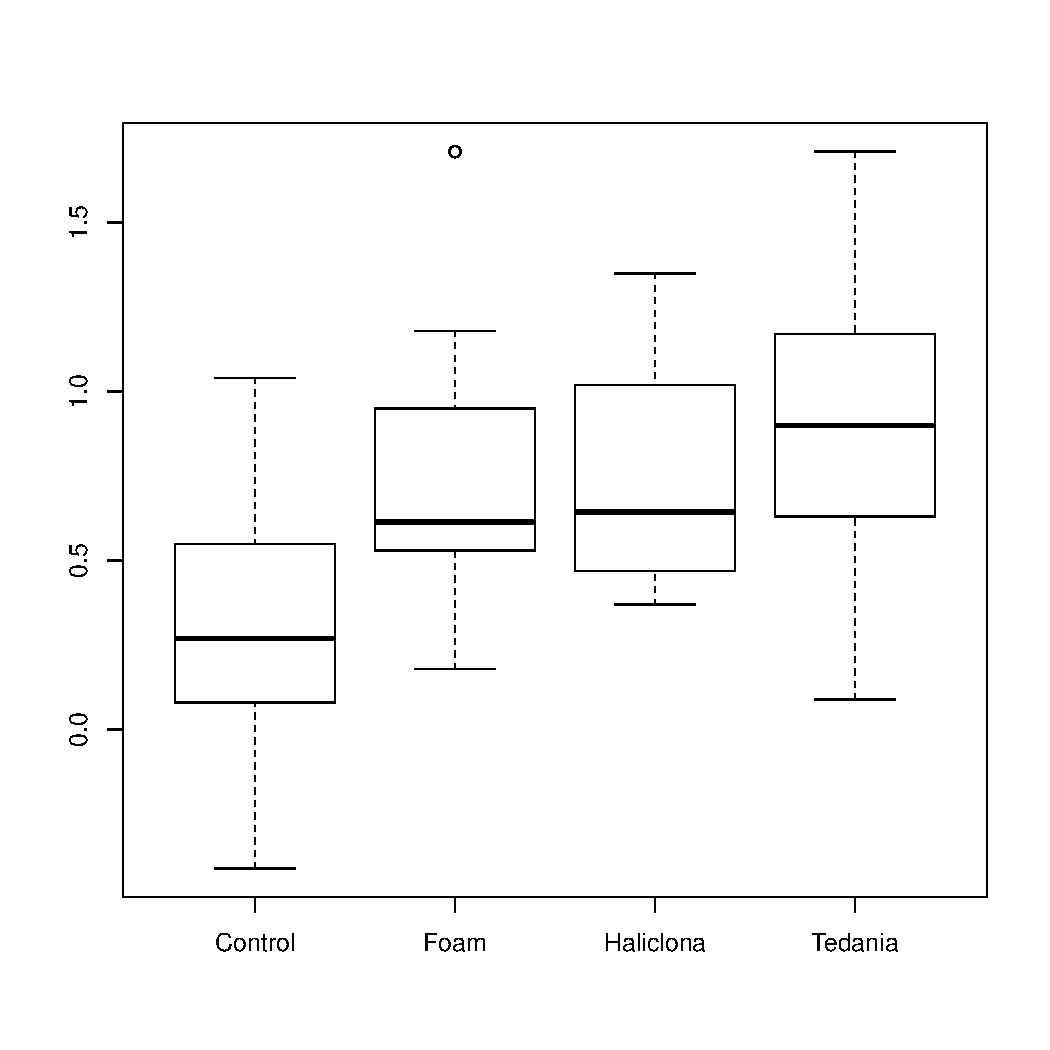
\includegraphics[width=0.6\linewidth]{figure/unnamed-chunk-4-1} 

\end{knitrout}

\end{frame}
%===============================================================================%

%===============================================================================%
\begin{frame}[fragile]{ANOVA: Exemplo}

\begin{knitrout}\tiny
\definecolor{shadecolor}{rgb}{0.969, 0.969, 0.969}\color{fgcolor}\begin{kframe}
\begin{alltt}
\hlstd{m1} \hlkwb{<-} \hlkwd{lm}\hlstd{(cresc} \hlopt{~} \hlstd{trat,mangue)}
\hlkwd{summary}\hlstd{(m1)}
\end{alltt}
\begin{verbatim}
## 
## Call:
## lm(formula = cresc ~ trat, data = mangue)
## 
## Residuals:
##      Min       1Q   Median       3Q      Max 
## -0.82357 -0.28643 -0.05786  0.24750  0.99786 
## 
## Coefficients:
##               Estimate Std. Error t value Pr(>|t|)    
## (Intercept)     0.3293     0.1083   3.040 0.003694 ** 
## tratFoam        0.3829     0.1532   2.500 0.015623 *  
## tratHaliclona   0.4357     0.1532   2.845 0.006341 ** 
## tratTedania     0.5843     0.1532   3.815 0.000363 ***
## ---
## Signif. codes:  0 '***' 0.001 '**' 0.01 '*' 0.05 '.' 0.1 ' ' 1
## 
## Residual standard error: 0.4052 on 52 degrees of freedom
## Multiple R-squared:  0.2335,	Adjusted R-squared:  0.1893 
## F-statistic: 5.281 on 3 and 52 DF,  p-value: 0.002963
\end{verbatim}
\end{kframe}
\end{knitrout}

\end{frame}
%===============================================================================%

%===============================================================================%
\begin{frame}[fragile]{ANOVA: Exemplo}

\begin{knitrout}\tiny
\definecolor{shadecolor}{rgb}{0.969, 0.969, 0.969}\color{fgcolor}\begin{kframe}
\begin{alltt}
\hlkwd{anova}\hlstd{(m1)}
\end{alltt}
\begin{verbatim}
## Analysis of Variance Table
## 
## Response: cresc
##           Df Sum Sq Mean Sq F value   Pr(>F)   
## trat       3 2.6014 0.86713  5.2807 0.002963 **
## Residuals 52 8.5388 0.16421                    
## ---
## Signif. codes:  0 '***' 0.001 '**' 0.01 '*' 0.05 '.' 0.1 ' ' 1
\end{verbatim}
\end{kframe}
\end{knitrout}

\end{frame}
%===============================================================================%

%===============================================================================%
\begin{frame}[fragile]{ANOVA: Exemplo}

\begin{knitrout}\tiny
\definecolor{shadecolor}{rgb}{0.969, 0.969, 0.969}\color{fgcolor}\begin{kframe}
\begin{alltt}
\hlstd{m1} \hlkwb{<-} \hlkwd{aov}\hlstd{(cresc} \hlopt{~} \hlstd{trat,mangue)}
\hlkwd{summary}\hlstd{(m1)}
\end{alltt}
\begin{verbatim}
##             Df Sum Sq Mean Sq F value  Pr(>F)   
## trat         3  2.601  0.8671   5.281 0.00296 **
## Residuals   52  8.539  0.1642                   
## ---
## Signif. codes:  0 '***' 0.001 '**' 0.01 '*' 0.05 '.' 0.1 ' ' 1
\end{verbatim}
\begin{alltt}
\hlkwd{anova}\hlstd{(m1)}
\end{alltt}
\begin{verbatim}
## Analysis of Variance Table
## 
## Response: cresc
##           Df Sum Sq Mean Sq F value   Pr(>F)   
## trat       3 2.6014 0.86713  5.2807 0.002963 **
## Residuals 52 8.5388 0.16421                    
## ---
## Signif. codes:  0 '***' 0.001 '**' 0.01 '*' 0.05 '.' 0.1 ' ' 1
\end{verbatim}
\end{kframe}
\end{knitrout}

\end{frame}
%===============================================================================%

%===============================================================================%
\begin{frame}[fragile]{ANOVA: Exemplo}

\begin{knitrout}\tiny
\definecolor{shadecolor}{rgb}{0.969, 0.969, 0.969}\color{fgcolor}\begin{kframe}
\begin{alltt}
\hlcom{# O teste F sugere uma diferença "significativa"...mas entre quais tratamentos?}
\hlkwd{TukeyHSD}\hlstd{(m1)}
\end{alltt}
\begin{verbatim}
##   Tukey multiple comparisons of means
##     95% family-wise confidence level
## 
## Fit: aov(formula = cresc ~ trat, data = mangue)
## 
## $trat
##                         diff         lwr       upr     p adj
## Foam-Control      0.38285714 -0.02364685 0.7893611 0.0717335
## Haliclona-Control 0.43571429  0.02921029 0.8422183 0.0312321
## Tedania-Control   0.58428571  0.17778172 0.9907897 0.0020035
## Haliclona-Foam    0.05285714 -0.35364685 0.4593611 0.9857121
## Tedania-Foam      0.20142857 -0.20507542 0.6079326 0.5576368
## Tedania-Haliclona 0.14857143 -0.25793257 0.5550754 0.7669696
\end{verbatim}
\end{kframe}
\end{knitrout}

\end{frame}
%===============================================================================%

%===============================================================================%
\begin{frame}[fragile]{ANOVA: Exemplo}

\begin{knitrout}\tiny
\definecolor{shadecolor}{rgb}{0.969, 0.969, 0.969}\color{fgcolor}\begin{kframe}
\begin{alltt}
\hlcom{# Testes pareados geram um pouco de confusão...}
\hlcom{# Melhor usar contrastes!}
\hlcom{#}
\hlcom{# Será que esponjas tem um efeito diferente da espuma artificial? (0,2,-1,-1)}
\hlstd{c1} \hlkwb{<-} \hlkwd{c}\hlstd{(}\hlkwd{rep}\hlstd{(}\hlnum{0}\hlstd{,}\hlnum{14}\hlstd{),}\hlkwd{rep}\hlstd{(}\hlnum{2}\hlstd{,}\hlnum{14}\hlstd{),}\hlkwd{rep}\hlstd{(}\hlopt{-}\hlnum{1}\hlstd{,}\hlnum{28}\hlstd{))}
\hlstd{mangue}\hlopt{$}\hlstd{c1} \hlkwb{<-} \hlstd{c1}
\hlstd{m2} \hlkwb{<-} \hlkwd{lm}\hlstd{(cresc} \hlopt{~} \hlstd{c1, mangue)}
\hlkwd{anova}\hlstd{(m2)}
\end{alltt}
\begin{verbatim}
## Analysis of Variance Table
## 
## Response: cresc
##           Df  Sum Sq Mean Sq F value Pr(>F)
## c1         1  0.1509 0.15088  0.7414  0.393
## Residuals 54 10.9893 0.20351
\end{verbatim}
\end{kframe}
\end{knitrout}

\end{frame}
%===============================================================================%


%===============================================================================%
\begin{frame}[fragile]{ANOVA: Exemplo}

\begin{knitrout}\tiny
\definecolor{shadecolor}{rgb}{0.969, 0.969, 0.969}\color{fgcolor}\begin{kframe}
\begin{alltt}
\hlcom{# Testando múltiplas hipóteses usando contrastes}

\hlcom{# 1) Será que esponjas tem um efeito diferente da espuma artificial? (0,2,-1,-1)}

\hlcom{# 2) Será que a adição de eponja/espuma faz diferença em relação ao controle? (3,-1,-1,-1)}

\hlcom{# 3) Será que existe diferença entre Tedania e Haliclonia? (0,1,-1,-1)}

\hlcom{# 4) Será que...opa! Só podemos usar até r-1 contrastes, e r = 4!}

\hlstd{c2} \hlkwb{<-} \hlkwd{c}\hlstd{(}\hlkwd{rep}\hlstd{(}\hlnum{3}\hlstd{,}\hlnum{14}\hlstd{),}\hlkwd{rep}\hlstd{(}\hlopt{-}\hlnum{1}\hlstd{,}\hlnum{42}\hlstd{))}
\hlstd{c3} \hlkwb{<-} \hlkwd{c}\hlstd{(}\hlkwd{rep}\hlstd{(}\hlnum{0}\hlstd{,}\hlnum{28}\hlstd{),}\hlkwd{rep}\hlstd{(}\hlnum{1}\hlstd{,}\hlnum{14}\hlstd{),}\hlkwd{rep}\hlstd{(}\hlopt{-}\hlnum{1}\hlstd{,}\hlnum{14}\hlstd{))}

\hlstd{mangue}\hlopt{$}\hlstd{c2} \hlkwb{<-} \hlstd{c2}
\hlstd{mangue}\hlopt{$}\hlstd{c3} \hlkwb{<-} \hlstd{c3}

\hlkwd{sum}\hlstd{(mangue}\hlopt{$}\hlstd{c1}\hlopt{*}\hlstd{mangue}\hlopt{$}\hlstd{c2}\hlopt{*}\hlstd{mangue}\hlopt{$}\hlstd{c3)}
\end{alltt}
\begin{verbatim}
## [1] 0
\end{verbatim}
\end{kframe}
\end{knitrout}

\end{frame}
%===============================================================================%

%===============================================================================%
\begin{frame}[fragile]{ANOVA: Exemplo}

\begin{knitrout}\tiny
\definecolor{shadecolor}{rgb}{0.969, 0.969, 0.969}\color{fgcolor}\begin{kframe}
\begin{alltt}
\hlcom{# Testando múltiplas hipóteses usando contrastes}

\hlcom{# 1) Será que esponjas tem um efeito diferente da espuma artificial? (0,2,-1,-1)}

\hlcom{# 2) Será que a adição de eponja/espuma faz diferença em relação ao controle? (3,-1,-1,-1)}

\hlcom{# 3) Será que existe diferença entre Tedania e Haliclonia? (0,1,-1,-1)}

\hlstd{m3} \hlkwb{<-} \hlkwd{lm}\hlstd{(cresc} \hlopt{~} \hlstd{c1} \hlopt{+} \hlstd{c2} \hlopt{+} \hlstd{c3, mangue)}

\hlkwd{anova}\hlstd{(m3)}
\end{alltt}
\begin{verbatim}
## Analysis of Variance Table
## 
## Response: cresc
##           Df Sum Sq Mean Sq F value   Pr(>F)    
## c1         1 0.1509 0.15088  0.9188 0.342223    
## c2         1 2.2960 2.29601 13.9824 0.000461 ***
## c3         1 0.1545 0.15451  0.9410 0.336519    
## Residuals 52 8.5388 0.16421                     
## ---
## Signif. codes:  0 '***' 0.001 '**' 0.01 '*' 0.05 '.' 0.1 ' ' 1
\end{verbatim}
\end{kframe}
\end{knitrout}

\end{frame}
%===============================================================================%

%===============================================================================%
\begin{frame}[fragile]{ANOVA: Exemplo}

\begin{knitrout}\tiny
\definecolor{shadecolor}{rgb}{0.969, 0.969, 0.969}\color{fgcolor}\begin{kframe}
\begin{alltt}
\hlcom{# Qual o efeito prático de se usarem diferentes contrastes?}
\hlcom{# Obter diferentes partições de variância!}
\hlkwd{anova}\hlstd{(m3)}
\end{alltt}
\begin{verbatim}
## Analysis of Variance Table
## 
## Response: cresc
##           Df Sum Sq Mean Sq F value   Pr(>F)    
## c1         1 0.1509 0.15088  0.9188 0.342223    
## c2         1 2.2960 2.29601 13.9824 0.000461 ***
## c3         1 0.1545 0.15451  0.9410 0.336519    
## Residuals 52 8.5388 0.16421                     
## ---
## Signif. codes:  0 '***' 0.001 '**' 0.01 '*' 0.05 '.' 0.1 ' ' 1
\end{verbatim}
\begin{alltt}
\hlkwd{anova}\hlstd{(m3)[}\hlnum{1}\hlopt{:}\hlnum{3}\hlstd{,}\hlnum{2}\hlstd{]}
\end{alltt}
\begin{verbatim}
## [1] 0.1508762 2.2960095 0.1545143
\end{verbatim}
\begin{alltt}
\hlkwd{sum}\hlstd{(}\hlkwd{anova}\hlstd{(m3)[}\hlnum{1}\hlopt{:}\hlnum{3}\hlstd{,}\hlnum{2}\hlstd{])}
\end{alltt}
\begin{verbatim}
## [1] 2.6014
\end{verbatim}
\end{kframe}
\end{knitrout}

\end{frame}
%===============================================================================%

%===============================================================================%
\begin{frame}[fragile]{ANOVA: Exemplo}

\begin{knitrout}\tiny
\definecolor{shadecolor}{rgb}{0.969, 0.969, 0.969}\color{fgcolor}\begin{kframe}
\begin{alltt}
\hlcom{# Qual o efeito prático de se usarem diferentes contrastes?}
\hlcom{# Obter diferentes partições de variância!}
\hlkwd{sum}\hlstd{(}\hlkwd{anova}\hlstd{(m3)[}\hlnum{1}\hlopt{:}\hlnum{3}\hlstd{,}\hlnum{2}\hlstd{])}
\end{alltt}
\begin{verbatim}
## [1] 2.6014
\end{verbatim}
\begin{alltt}
\hlkwd{anova}\hlstd{(m1)}
\end{alltt}
\begin{verbatim}
## Analysis of Variance Table
## 
## Response: cresc
##           Df Sum Sq Mean Sq F value   Pr(>F)   
## trat       3 2.6014 0.86713  5.2807 0.002963 **
## Residuals 52 8.5388 0.16421                    
## ---
## Signif. codes:  0 '***' 0.001 '**' 0.01 '*' 0.05 '.' 0.1 ' ' 1
\end{verbatim}
\end{kframe}
\end{knitrout}

\end{frame}
%===============================================================================%

%===============================================================================%
\begin{frame}{ANOVA: modelos com efeitos fixos e aleatórios}

Uma importante distinção ao se realizar uma ANOVA é quanto ao tipo de efeito do tratamento:
\vfill

\begin{block}{Efeito Fixo:}
$r$ representa o conjunto completo de todos os níveis de interesse possíveis, ou seja, uma população. Exemplo: Temos quatro alunos de estatística, será que o desempenho ao longo do curso foi diferente para cada um destes quatro?
\end{block}
\vfill

\pause

\begin{block}{Efeito Aleatório:}
$r$ representa um subconjunto de todos os níveis possíves de $X$, ou seja, uma amostra. Será que existe variação na performance dos alunos de Estatística, com base nesses quatro que eu observei? 
\end{block}
\vfill

\end{frame}
%===============================================================================%


%===============================================================================%
\begin{frame}{ANOVA: modelos com efeitos fixos e aleatórios}

A classificação dos efeitos se dá em função do tipo de inferência que se espera fazer para os níveis: \pause
\vfill

\textbf{``Aluno'' como fator de efeito fixo:} estamos preocupados em inferir se existem diferenças entre os quatro alunos especificados, em termos de desempenho. \pause
\vfill

\textbf{``Aluno'' como fator de efeito aleatório:} estamos preocupados em inferir se existe varição no desempenho dos alunos em geral, no curso de de estatística. Os quatro alunos avaliados são uma amostra aleatória do universo de todos os possíveis alunos da disciplina.
\end{frame}
%===============================================================================%


%===============================================================================%
\begin{frame}{ANOVA: efeitos aleatórios}

Quando os níveis de $X$ são aleatórios, o modelo é espcificado da mesma maneira: 
\vfill
$Y_{ij} = \mu + \alpha_i + \epsilon _{ij}$ \pause
\vfill
A grande diferença é que $\alpha$ agora vem de um valor aleatório, e por isso tem uma distribuição com média e variância:
\vfill
$\alpha _i \sim N(0,\sigma ^2 _\alpha)$ \pause
\vfill
E o nosso modelo agora depende de duas variâncias: $\sigma ^2$ e $\sigma ^2 _\alpha$

\end{frame}
%===============================================================================%


%===============================================================================%
\begin{frame}{ANOVA: efeitos aleatórios}

O mais importante, contudo, é que nossa hipótese nula é bastante diferente. \pause
\vfill
Para o modelo de efeitos fixos, queremos avaliar se:
$\alpha _1 = \alpha _2 = \ldots = \alpha _i$ (não há diferença entre tratamentos) \pause
\vfill
Mas para o modelo de efeitos aleatórios, queremos avaliar se:
\vfill
$\sigma ^2 _\alpha = 0$ (não há variação entre os diferentes tratamentos) \pause
\vfill
De fato, no modelo aleatório, não faz sentido testar diferenças entre tratamentos: a cada nova realização do experimento, esses tratamentos seriam diferentes! 
\end{frame}
%===============================================================================%

%===============================================================================%
\begin{frame}{ANOVA: Teste de hipóteses para efeitos aleatórios}

Para o modelo ANOVA com efeitos aleatórios, $E(MQ_{Reg})$ é:
\vfill

$ r\sigma ^2 _\alpha + \sigma ^2$ \pause
\vfill

E ainda temos $E(MQ_{Res}) = \sigma^2$  \pause
\vfill

Se todos os níveis do fator são iguais, então $\sigma ^2 _\alpha = 0$ e temos:

\begin{equation*}
F = \frac{MQ_{Reg}}{MQ_{Res}} =  \frac{r\sigma ^2 _\alpha + \sigma ^2}{\sigma ^2} = \frac{\sigma^2}{\sigma^2} = 1
\end{equation*}
\vfill \pause
Mas se os níveis são diferentes, então $\sigma ^2 _\alpha > 0$, e $F > 1$
\vfill
\textbf{Importante:} O teste F para ANOVA com efeitos fixos e aleatórios é igual apenas para análises com um um unico fator.

\end{frame}
%===============================================================================%

%===============================================================================%
\begin{frame}{ANCOVA}

\textbf{ANCOVA:} Análise de Covariância
\vfill
\begin{itemize}
\item Uma ``mistura'' de regressão e ANOVA
\vfill
\item Mistura variáveis explicativas categóricas (\emph{dummy}) e contínuas
\vfill
\item Pode incluir termos de \texbf{interação}
\vfill
\item $ Y = \beta _0 + \beta _1 X_1 + \beta _2 X_2 + \mathbf{ \boldsymbol{\beta} _3 X_1X_2} + \varepsilon$
\vfill
\end{itemize}

\end{frame}
%===============================================================================%


%===============================================================================%
\begin{frame}{ANOVA Multifatorial}

Extensão da ANOVA para mais de uma variável explicativa (todas categóricas)
\vfill
\begin{itemize}
\item Geralmente também inclui termos de interação.
\vfill
\item Com três ou mais fatores, a interpretação fica bastante difícil.
\vfill
\item Fortemente baseada em desenhos experimentais controlados, que permitam a partição correta da variância, sem multicolinearidade ou pseudoreplicação.
\vfill
\end{itemize}

\end{frame}
%===============================================================================%


%===============================================================================%
\begin{frame}{ANCOVA}

\begin{small}

A variável categórica altera o intercepto ($X_2 =(0,1)$)  :

\begin{equation*}
Y = \beta _0 + \beta _1 X_1 + \beta _2 X_2 + \varepsilon
\end{equation*}

Para o nível 1 de $X_2$:

\begin{equation*}
Y = \beta _0 + \beta _1 X_1 + \beta _2 \times 0 + \varepsilon = \beta _0 + \beta _1 X_1 + \varepsilon
\end{equation*}

Para o nível 2 de $X_2$:

\begin{equation*}
Y = \beta _0 + \beta _1 X_1 + \beta _2 \times 1 + \varepsilon
\end{equation*}

\begin{equation*}
Y = (\beta _0 + \beta _2) +  \beta _1 X_1 + \varepsilon
\end{equation*}

\end{small}

\end{frame}
%===============================================================================%



%===============================================================================%
\begin{frame}[fragile]{ANCOVA}

\begin{columns}

\column{0.65\linewidth}
\setlength{\topsep}{2pt}
\begin{knitrout}\tiny
\definecolor{shadecolor}{rgb}{0.969, 0.969, 0.969}\color{fgcolor}\begin{kframe}
\begin{alltt}
\hlkwd{set.seed}\hlstd{(}\hlnum{234}\hlstd{)}
\hlstd{x1} \hlkwb{<-} \hlkwd{runif}\hlstd{(}\hlnum{40}\hlstd{,}\hlnum{0}\hlstd{,}\hlnum{20}\hlstd{)}
\hlstd{x2} \hlkwb{<-} \hlkwd{c}\hlstd{(}\hlkwd{rep}\hlstd{(}\hlnum{0}\hlstd{,}\hlnum{20}\hlstd{),}\hlkwd{rep}\hlstd{(}\hlnum{1}\hlstd{,}\hlnum{20}\hlstd{))}
\hlstd{col} \hlkwb{<-} \hlstd{x2; col[col}\hlopt{==}\hlnum{0}\hlstd{]} \hlkwb{<-} \hlstr{"blue"}\hlstd{; col[col}\hlopt{==}\hlnum{1}\hlstd{]} \hlkwb{<-} \hlstr{"red"}
\hlstd{y} \hlkwb{<-} \hlnum{3} \hlopt{+} \hlnum{2}\hlopt{*}\hlstd{x1} \hlopt{+} \hlnum{20}\hlopt{*}\hlstd{x2} \hlopt{+} \hlkwd{rnorm}\hlstd{(}\hlnum{20}\hlstd{,}\hlnum{0}\hlstd{,}\hlnum{5}\hlstd{)}

\hlstd{m} \hlkwb{<-} \hlkwd{lm}\hlstd{(y} \hlopt{~} \hlstd{x1} \hlopt{+} \hlstd{x2)}

\hlkwd{plot}\hlstd{(x1,y,} \hlkwc{pch}\hlstd{=}\hlnum{19}\hlstd{,}\hlkwc{col}\hlstd{=col)}

\hlstd{x21novo} \hlkwb{<-} \hlkwd{data.frame}\hlstd{(}\hlkwc{x1} \hlstd{=} \hlkwd{seq}\hlstd{(}\hlnum{0}\hlstd{,}\hlnum{20}\hlstd{,}\hlkwc{by}\hlstd{=}\hlnum{1}\hlstd{),} \hlkwc{x2}\hlstd{=}\hlkwd{rep}\hlstd{(}\hlnum{0}\hlstd{,}\hlnum{21}\hlstd{))}
\hlstd{x22novo} \hlkwb{<-} \hlkwd{data.frame}\hlstd{(}\hlkwc{x1} \hlstd{=} \hlkwd{seq}\hlstd{(}\hlnum{0}\hlstd{,}\hlnum{20}\hlstd{,}\hlkwc{by}\hlstd{=}\hlnum{1}\hlstd{),} \hlkwc{x2}\hlstd{=}\hlkwd{rep}\hlstd{(}\hlnum{1}\hlstd{,}\hlnum{21}\hlstd{))}

\hlstd{p1} \hlkwb{<-} \hlkwd{predict}\hlstd{(m,x21novo)}
\hlstd{p2} \hlkwb{<-} \hlkwd{predict}\hlstd{(m,x22novo)}

\hlkwd{lines}\hlstd{(}\hlkwd{seq}\hlstd{(}\hlnum{0}\hlstd{,}\hlnum{20}\hlstd{,}\hlkwc{by}\hlstd{=}\hlnum{1}\hlstd{),p1,} \hlkwc{lwd}\hlstd{=}\hlnum{2}\hlstd{,}\hlkwc{col}\hlstd{=}\hlstr{'blue'}\hlstd{)}
\hlkwd{lines}\hlstd{(}\hlkwd{seq}\hlstd{(}\hlnum{0}\hlstd{,}\hlnum{20}\hlstd{,}\hlkwc{by}\hlstd{=}\hlnum{1}\hlstd{),p2,} \hlkwc{lwd}\hlstd{=}\hlnum{2}\hlstd{,}\hlkwc{col}\hlstd{=}\hlstr{'red'}\hlstd{)}
\end{alltt}
\end{kframe}
\end{knitrout}

\column{0.4\linewidth}

\begin{knitrout}
\definecolor{shadecolor}{rgb}{0.969, 0.969, 0.969}\color{fgcolor}
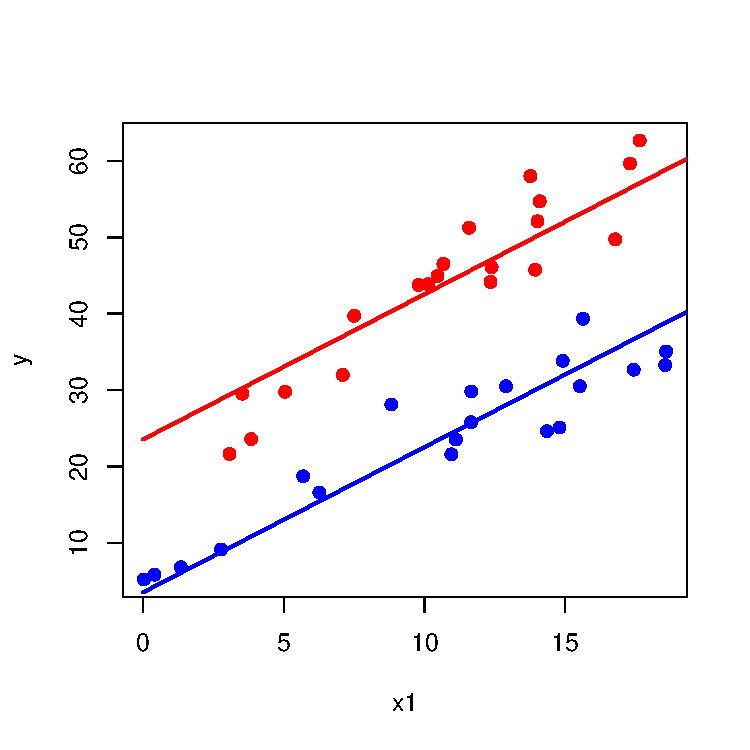
\includegraphics[width=1.1\linewidth]{figure/ancovplot1-1} 

\end{knitrout}


\end{columns}

\end{frame}
%===============================================================================%

%===============================================================================%
\begin{frame}[fragile]{ANCOVA}

\begin{columns}

\column{0.65\linewidth}
\setlength{\topsep}{2pt}
\begin{knitrout}\tiny
\definecolor{shadecolor}{rgb}{0.969, 0.969, 0.969}\color{fgcolor}\begin{kframe}
\begin{alltt}
\hlkwd{summary}\hlstd{(m)}
\end{alltt}
\begin{verbatim}
## 
## Call:
## lm(formula = y ~ x1 + x2)
## 
## Residuals:
##     Min      1Q  Median      3Q     Max 
## -7.7356 -3.4624  0.9155  2.5250  8.3066 
## 
## Coefficients:
##             Estimate Std. Error t value Pr(>|t|)    
## (Intercept)   3.5609     1.7138   2.078   0.0447 *  
## x1            1.8990     0.1323  14.358   <2e-16 ***
## x2           20.0080     1.3754  14.547   <2e-16 ***
## ---
## Signif. codes:  0 '***' 0.001 '**' 0.01 '*' 0.05 '.' 0.1 ' ' 1
## 
## Residual standard error: 4.349 on 37 degrees of freedom
## Multiple R-squared:  0.9192,	Adjusted R-squared:  0.9148 
## F-statistic: 210.5 on 2 and 37 DF,  p-value: < 2.2e-16
\end{verbatim}
\end{kframe}
\end{knitrout}

\column{0.4\linewidth}

\begin{knitrout}
\definecolor{shadecolor}{rgb}{0.969, 0.969, 0.969}\color{fgcolor}
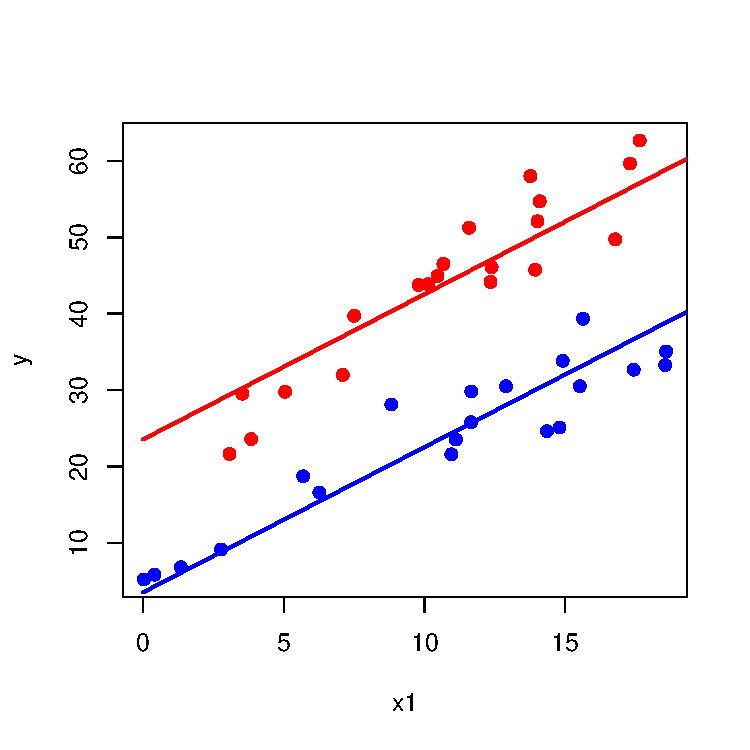
\includegraphics[width=1.1\linewidth]{figure/ancovplot2-1} 

\end{knitrout}


\end{columns}

\end{frame}
%===============================================================================%


%===============================================================================%
\begin{frame}{Mais algumas extensões dos Modelos Lineares Gerais}

\begin{small}

O termo de interação altera a inclinação:

\begin{equation*}
Y = \beta _0 + \beta _1 X_1 + \beta _2 X_2 + \beta _3 X_1 X_2 + \varepsilon
\end{equation*}

Para o nível 1 de $X_2$:

\begin{equation*}
Y = \beta _0  + \beta _1 X_1 + \beta _2 \times 0 + \beta _3 \times X_1 \times 0 + \varepsilon = Y = \beta _0 + \beta _1 X_1 + \varepsilon
\end{equation*}

Para o nível 2 de $X_2$:

\begin{equation*}
Y = \beta _0  + \beta _1 X_1 + \beta _2 \times 1 + \beta _3 \times X_1 \times 1 + \varepsilon
\end{equation*}

\begin{equation*}
Y = (\beta _0 +  \beta _2) + (\beta _1 + \beta _3) \times  X_1 + \varepsilon
\end{equation*}

\end{small}

\end{frame}
%===============================================================================%



%===============================================================================%
\begin{frame}[fragile]{ANCOVA}

\begin{columns}

\column{0.65\linewidth}
\setlength{\topsep}{2pt}
\begin{knitrout}\tiny
\definecolor{shadecolor}{rgb}{0.969, 0.969, 0.969}\color{fgcolor}\begin{kframe}
\begin{alltt}
\hlkwd{set.seed}\hlstd{(}\hlnum{234}\hlstd{)}
\hlstd{x1} \hlkwb{<-} \hlkwd{runif}\hlstd{(}\hlnum{40}\hlstd{,}\hlnum{0}\hlstd{,}\hlnum{20}\hlstd{)}
\hlstd{x2} \hlkwb{<-} \hlkwd{c}\hlstd{(}\hlkwd{rep}\hlstd{(}\hlnum{0}\hlstd{,}\hlnum{20}\hlstd{),}\hlkwd{rep}\hlstd{(}\hlnum{1}\hlstd{,}\hlnum{20}\hlstd{))}
\hlstd{y} \hlkwb{<-} \hlnum{3} \hlopt{+} \hlnum{2}\hlopt{*}\hlstd{x1} \hlopt{+} \hlnum{6}\hlopt{*}\hlstd{x2} \hlopt{+} \hlnum{1.2}\hlopt{*}\hlstd{x1}\hlopt{*}\hlstd{x2} \hlopt{+} \hlkwd{rnorm}\hlstd{(}\hlnum{20}\hlstd{,}\hlnum{0}\hlstd{,}\hlnum{5}\hlstd{)}

\hlstd{m} \hlkwb{<-} \hlkwd{lm}\hlstd{(y} \hlopt{~} \hlstd{x1} \hlopt{*} \hlstd{x2)}

\hlstd{m} \hlkwb{<-} \hlkwd{lm}\hlstd{(y} \hlopt{~} \hlstd{x1} \hlopt{*} \hlstd{x2)}

\hlstd{x21novo} \hlkwb{<-} \hlkwd{data.frame}\hlstd{(}\hlkwc{x1} \hlstd{=} \hlkwd{seq}\hlstd{(}\hlnum{0}\hlstd{,}\hlnum{20}\hlstd{,}
                \hlkwc{by}\hlstd{=}\hlnum{1}\hlstd{),} \hlkwc{x2}\hlstd{=}\hlkwd{rep}\hlstd{(}\hlnum{0}\hlstd{,}\hlnum{21}\hlstd{))}
\hlstd{x22novo} \hlkwb{<-} \hlkwd{data.frame}\hlstd{(}\hlkwc{x1} \hlstd{=} \hlkwd{seq}\hlstd{(}\hlnum{0}\hlstd{,}\hlnum{20}
                       \hlstd{,}\hlkwc{by}\hlstd{=}\hlnum{1}\hlstd{),} \hlkwc{x2}\hlstd{=}\hlkwd{rep}\hlstd{(}\hlnum{1}\hlstd{,}\hlnum{21}\hlstd{))}

\hlstd{p1} \hlkwb{<-} \hlkwd{predict}\hlstd{(m,x21novo)}
\hlstd{p2} \hlkwb{<-} \hlkwd{predict}\hlstd{(m,x22novo)}

\hlkwd{plot}\hlstd{(x1,y,} \hlkwc{pch}\hlstd{=}\hlnum{19}\hlstd{,} \hlkwc{col}\hlstd{=col)}

\hlkwd{lines}\hlstd{(}\hlkwd{seq}\hlstd{(}\hlnum{0}\hlstd{,}\hlnum{20}\hlstd{,}\hlkwc{by}\hlstd{=}\hlnum{1}\hlstd{),p1,} \hlkwc{lwd}\hlstd{=}\hlnum{2}\hlstd{,}\hlkwc{col}\hlstd{=}\hlstr{'blue'}\hlstd{)}
\hlkwd{lines}\hlstd{(}\hlkwd{seq}\hlstd{(}\hlnum{0}\hlstd{,}\hlnum{20}\hlstd{,}\hlkwc{by}\hlstd{=}\hlnum{1}\hlstd{),p2,} \hlkwc{lwd}\hlstd{=}\hlnum{2}\hlstd{,}\hlkwc{col}\hlstd{=}\hlstr{'red'}\hlstd{)}
\end{alltt}
\end{kframe}
\end{knitrout}

\column{0.4\linewidth}

\begin{knitrout}
\definecolor{shadecolor}{rgb}{0.969, 0.969, 0.969}\color{fgcolor}
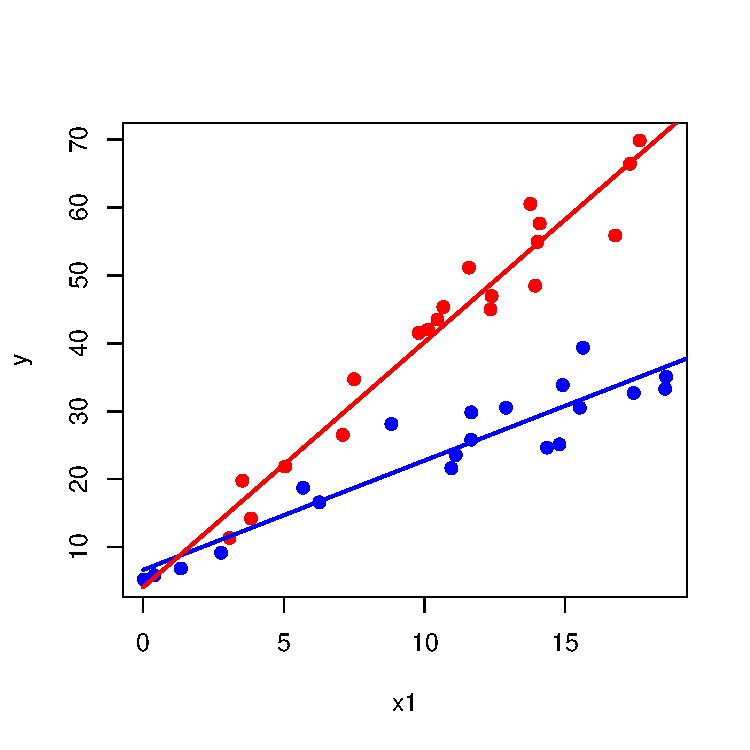
\includegraphics[width=1.1\linewidth]{figure/ancovplot3-1} 

\end{knitrout}


\end{columns}

\end{frame}
%===============================================================================%




%===============================================================================%
\begin{frame}[fragile]{ANCOVA}

\begin{columns}

\column{0.65\linewidth}
\setlength{\topsep}{2pt}
\begin{knitrout}\tiny
\definecolor{shadecolor}{rgb}{0.969, 0.969, 0.969}\color{fgcolor}\begin{kframe}
\begin{alltt}
\hlkwd{summary}\hlstd{(m)}
\end{alltt}
\begin{verbatim}
## 
## Call:
## lm(formula = y ~ x1 * x2)
## 
## Residuals:
##     Min      1Q  Median      3Q     Max 
## -8.7702 -2.1950 -0.2836  2.7892  7.5328 
## 
## Coefficients:
##             Estimate Std. Error t value Pr(>|t|)    
## (Intercept)   6.6411     1.7961   3.697 0.000721 ***
## x1            1.6103     0.1475  10.920 5.62e-13 ***
## x2           -2.5561     2.9011  -0.881 0.384121    
## x1:x2         1.9989     0.2453   8.149 1.09e-09 ***
## ---
## Signif. codes:  0 '***' 0.001 '**' 0.01 '*' 0.05 '.' 0.1 ' ' 1
## 
## Residual standard error: 3.875 on 36 degrees of freedom
## Multiple R-squared:  0.9511,	Adjusted R-squared:  0.947 
## F-statistic: 233.4 on 3 and 36 DF,  p-value: < 2.2e-16
\end{verbatim}
\end{kframe}
\end{knitrout}

\column{0.4\linewidth}

\begin{knitrout}
\definecolor{shadecolor}{rgb}{0.969, 0.969, 0.969}\color{fgcolor}
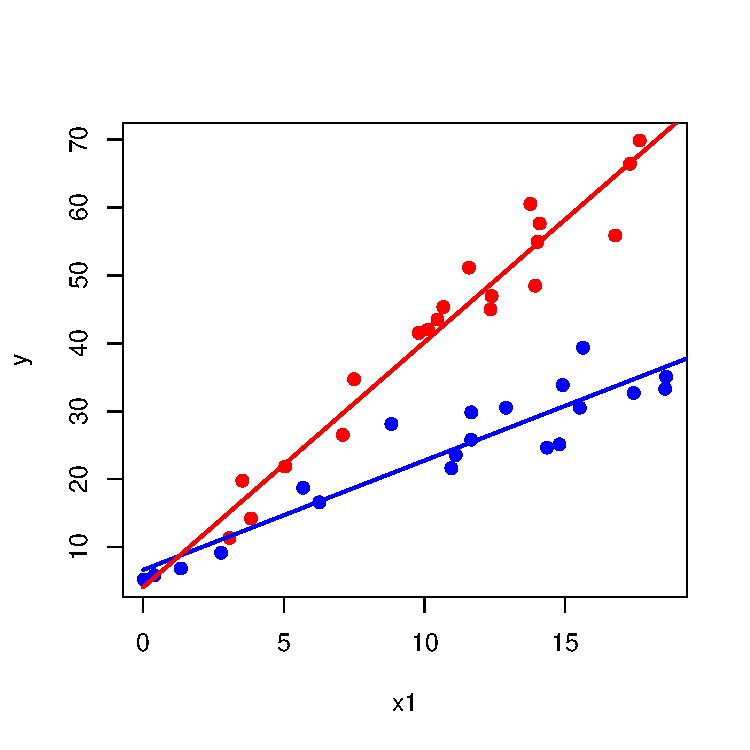
\includegraphics[width=1.1\linewidth]{figure/ancovplot4-1} 

\end{knitrout}


\end{columns}

\end{frame}
%===============================================================================%

%===============================================================================%
\begin{frame}[fragile]{ANCOVA}

\begin{columns}

\column{0.65\linewidth}
\setlength{\topsep}{2pt}
\begin{knitrout}\tiny
\definecolor{shadecolor}{rgb}{0.969, 0.969, 0.969}\color{fgcolor}\begin{kframe}
\begin{alltt}
\hlstd{m} \hlkwb{<-} \hlkwd{lm}\hlstd{(y} \hlopt{~} \hlstd{x1} \hlopt{+} \hlstd{x1}\hlopt{:}\hlstd{x2)}
\hlkwd{summary}\hlstd{(m)}
\end{alltt}
\begin{verbatim}
## 
## Call:
## lm(formula = y ~ x1 + x1:x2)
## 
## Residuals:
##     Min      1Q  Median      3Q     Max 
## -8.2419 -2.3296 -0.0221  2.7361  7.6408 
## 
## Coefficients:
##             Estimate Std. Error t value Pr(>|t|)    
## (Intercept)   5.6613     1.4062   4.026  0.00027 ***
## x1            1.6808     0.1235  13.607 5.63e-16 ***
## x1:x2         1.8030     0.1033  17.453  < 2e-16 ***
## ---
## Signif. codes:  0 '***' 0.001 '**' 0.01 '*' 0.05 '.' 0.1 ' ' 1
## 
## Residual standard error: 3.864 on 37 degrees of freedom
## Multiple R-squared:   0.95,	Adjusted R-squared:  0.9473 
## F-statistic: 351.8 on 2 and 37 DF,  p-value: < 2.2e-16
\end{verbatim}
\end{kframe}
\end{knitrout}

\column{0.4\linewidth}

\begin{knitrout}
\definecolor{shadecolor}{rgb}{0.969, 0.969, 0.969}\color{fgcolor}
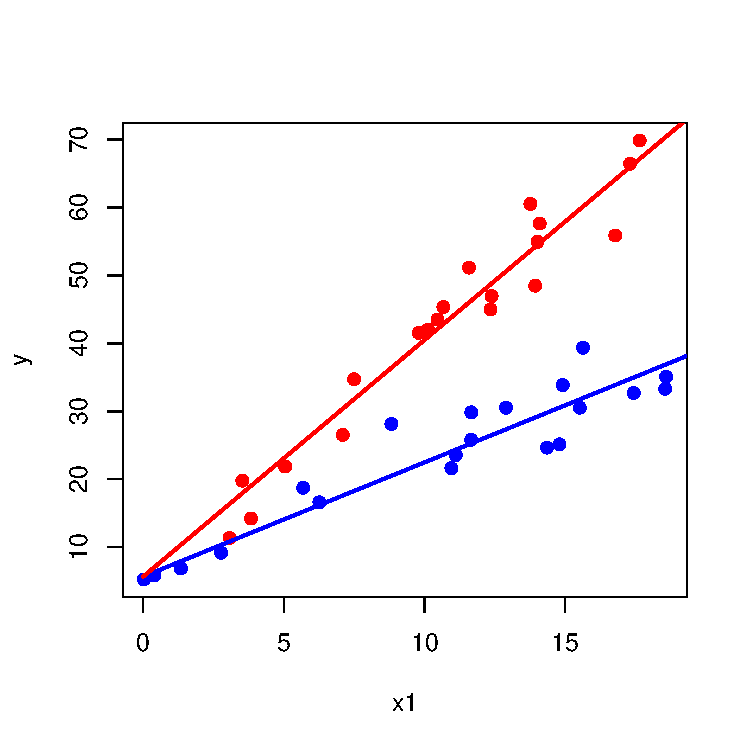
\includegraphics[width=1.1\linewidth]{figure/ancovplot5-1} 

\end{knitrout}


\end{columns}

\end{frame}
%===============================================================================%


%===============================================================================%
\begin{frame}{ANCOVA}

\begin{small}

Quando usar ANCOVA?
\vfill
\begin{itemize}
\item Explicar diferenças em uma relação contínua entre grupos (ex. fertilizante em duas espécies de planta) 
\vfill
\item O termo aditivo (novo intercepto) é interpretado como: mesma taxa de crescimento (inclinação), mas com níveis basais diferentes
\vfill
\item O termo de interação é intepretado como taxas (inclinações) diferentes. Ou seja, a resposta do fertilizante \emph{interage} com o tipo de espécie para determinar uma resposta.

\vfill
\item Se esses coeficientes são pequenos e/ou tem p-valor alto, interpreta-se que há pouca evidência de diferenças na relação entre $X_1$ e $Y$ para os diferentes grupos.
\end{itemize}

\end{small}

\end{frame}
%===============================================================================%

\end{document}
